%===============================================================================
% $Id: ifacconf.tex 19 2011-10-27 09:32:13Z jpuente $  
% Template for IFAC meeting papers
% Copyright (c) 2007-2008 International Federation of Automatic Control
%===============================================================================
\documentclass{ifacconf}

%\usepackage{graphicx}      % include this line if your document contains figures
\usepackage{natbib}        % required for bibliography

\usepackage[pdftex]{graphicx}
   \graphicspath{{./img/}}
   

\usepackage[usenames,dvipsnames]{xcolor}

\usepackage{amsmath} % assumes amsmath package installed
\usepackage{amssymb}  % assumes amsmath package installed

%---------------0---------------------
%---------------0---------------------
%---------------0---------------------
% USUNAC TE PAKIETY NA KONCU

%\usepackage{polski}
\usepackage[cp1250]{inputenc}
\usepackage[OT4]{fontenc}
%---------------0---------------------
%---------------0---------------------
%---------------0---------------------
%---------------0---------------------




%===============================================================================
\begin{document}
\begin{frontmatter}

%\title{Style for IFAC Conferences \& Symposia: Use Title Case for
%  Paper Title\thanksref{footnoteinfo}} 
\title{Hybrid controller for the Pendubot} 
% Title, preferably not more than 10 words.

%\thanks[footnoteinfo]{Sponsor and financial support acknowledgment
%goes here. Paper titles should be written in uppercase and lowercase
%letters, not all uppercase.}


\author[First]{Pawe\l{} Parulski} 
\author[Second]{Patryk Bartkowiak} 
\author[Third]{Dariusz Pazderski}
\author[Fourth]{Krzysztof Koz\l{}owski}

\address[First]{Institute of Automation and Robotics, 
   Poznan University of Technology, Poznan, Poland 
   (e-mail: pawel.parulski@put.poznan.pl).}
\address[Second]{Institute of Automation and Robotics, 
   Poznan University of Technology, Poznan, Poland 
   (e-mail: author@put.poznan.pl)}
\address[Third]{Institute of Automation and Robotics, 
   Poznan University of Technology, Poznan, Poland  
   (e-mail: author@put.poznan.pl)}
\address[Fourth]{Institute of Automation and Robotics, 
   Poznan University of Technology, Poznan, Poland  
   (e-mail: author@put.poznan.pl)}

\begin{abstract}                % Abstract of not more than 250 words.
The aim of this paper is to
test the usefulness of a new approach based on  partial feedback linearisation to control the Pendubot.
%
The control problem stated in the article is to stabilize the Pendubot in the upright position.
\end{abstract}

\begin{keyword}
Robotics, Robot dynamics, Pendubot, nonlinear control, feedback linearization, nonlinearity, 
%Five to ten keywords, preferably chosen from the IFAC keyword list.
\end{keyword}

\end{frontmatter}
%===============================================================================

\section{Introduction}

Acrobot and Pendubot are well-known fundamental examples of underactuated planar mechanical systems moving in the presence of the gravity. Although their kinematic structures are relatively simple, still they can be considered as important benchmark systems which are of great importance for the development of nonlinear control strategies. 

Basically, a standard approach to stabilise both systems at an unstable equilibrium requires design of two controllers for the task of swing-up (when the robot hangs down) and the balancing task around the equilibrium point, respectively.

Many solutions to the first problem are based on the work of \cite{Spong_partial, xin_swing_new}, the second, is still being developed by many authors.

The control of double inverted pendulum is still an open problem. Recently, in \cite{Respondek_2019} a new insight to control of underactuated systems is investigated. The proposed concept is to find the largest feedback linearizable subsystem for mechanical systems that are not feedback linearizable. Basically, the authors of this paper ore focused on the problem of choosing a partially linearizing output that renders the zero dynamics asymptotically stable,
and illustrate the theoretical results by mathematical formulas developed for double inverted pendulum with one actuator (Acrobot and Pendubot). However, no attempt is done  to use the discussed concept to design a controller for these benchmark systems. Hence, any simulation or experimental verification has not been reported yet.
%
In this paper authors attempt to fill this gap and extend preliminary results recently discussed by \cite{bartkowiak} for the Pendubot. Authors are also interested in the applicability of such an algorithm to the physically existing root.

The paper is organized as follows. Section \ref{sec:modelowanie} describes the mathematical model for the Pendubot system, together with constrains imposed on the model. 
%
In section \ref{sec:stabilization_problem} the analysed control algorithms along with the state transformation for the stabilization task is introduced.
%
Section \ref{sec:symulacje_i_porowanie} describes the simulation results of analysed algorithms, while the Section \ref{sec:konkluzje} gives final remarks.



% % % % % % % % % % % % % % % % % % % % % % % % % % % % % %


\section{Model}
\label{sec:modelowanie}

The Pendubot is a connection of  $N = 2$ rigid bodies coupled  in a tree structure, supported on ground via an actuated frictionless revolute joint. Both links have non-zero mass and the revolute joint connecting them is unactuated. As a result, the system has one degree of underactuation ($2$ DOF with $1$ independent actuator).
%
\begin{figure}[!ht]
\centering
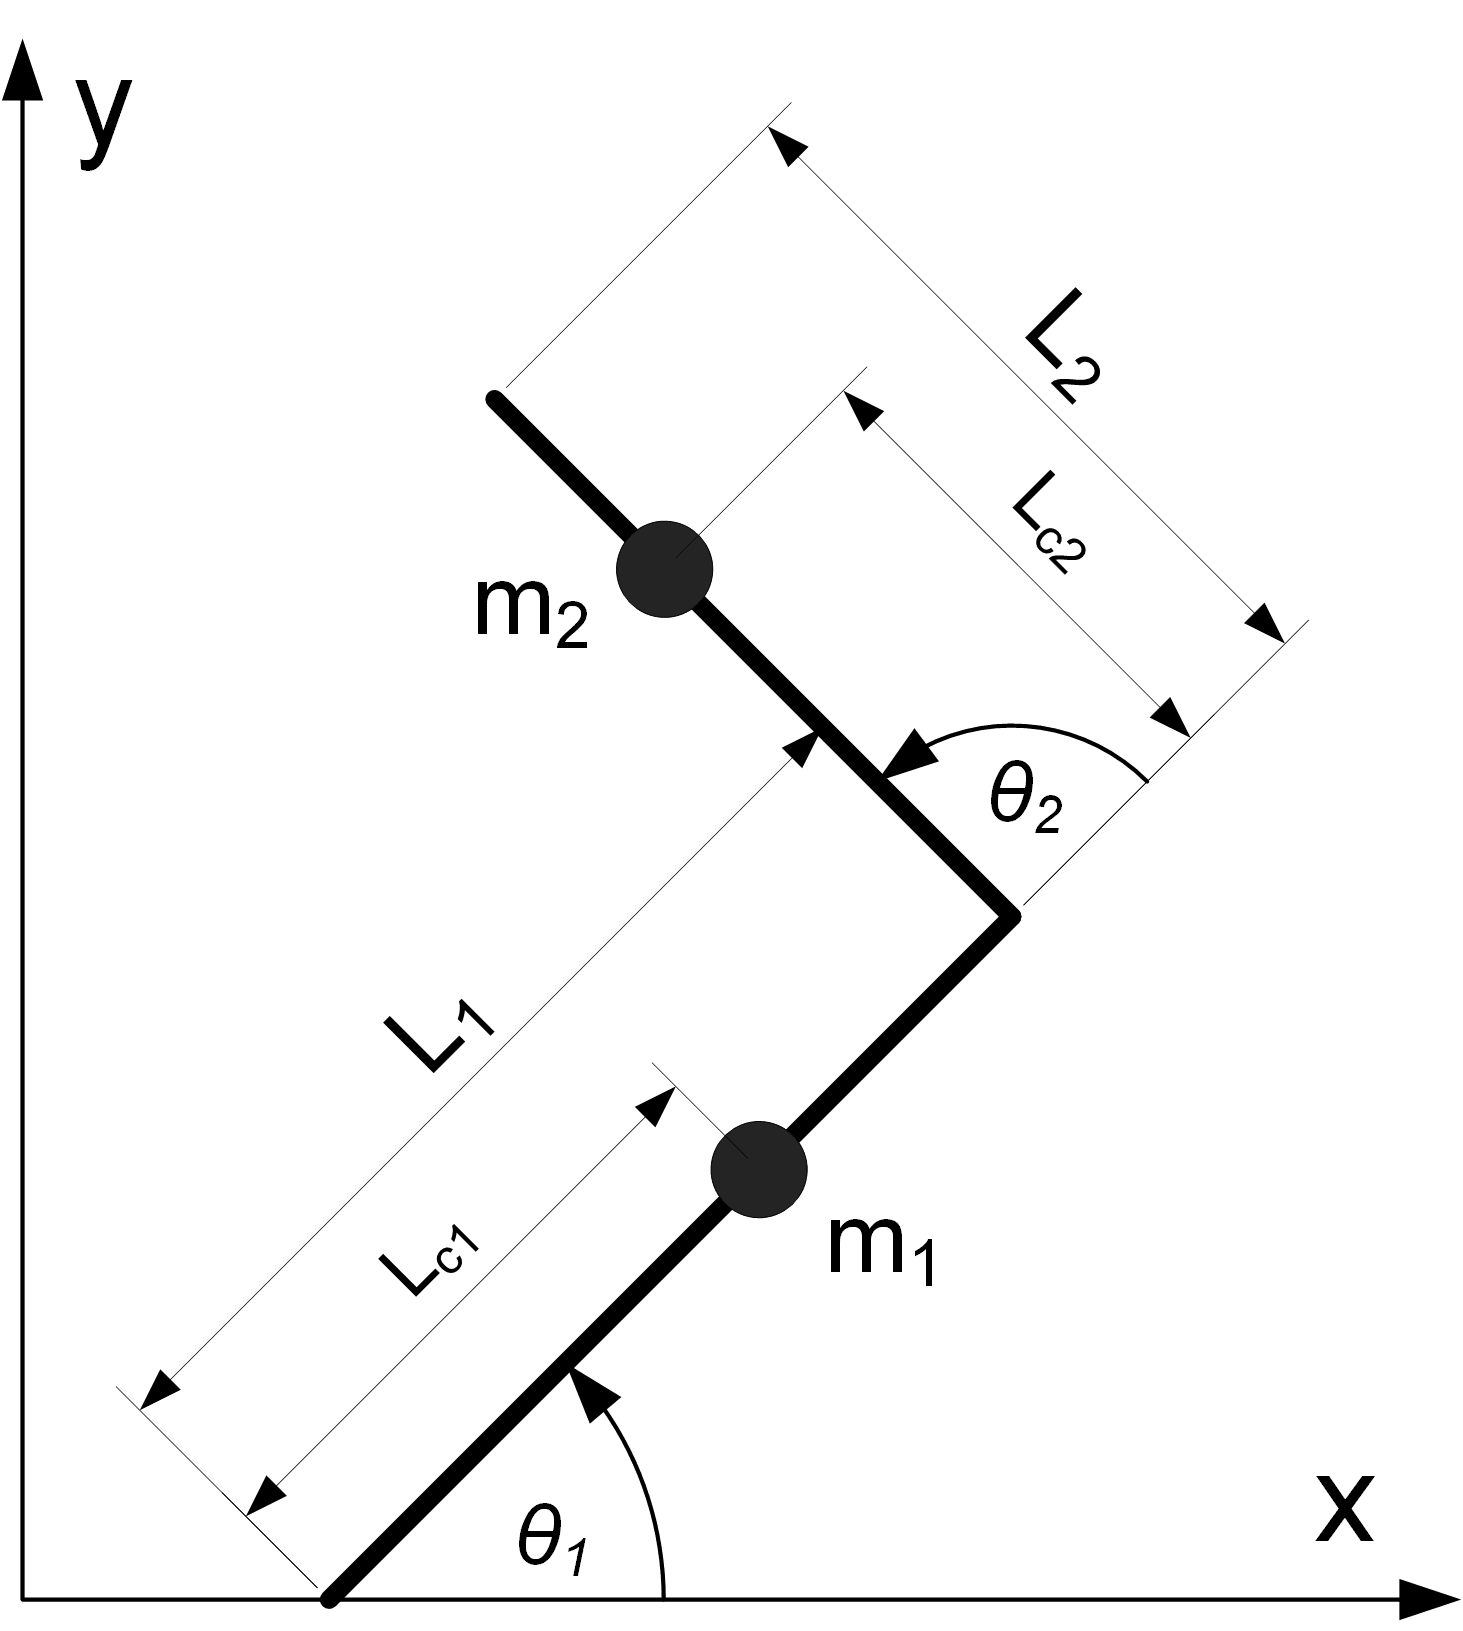
\includegraphics[height=0.3\textwidth]{2_link}
\caption{Two link inverted pendulum, with one actuator -- Pendubot}
\label{fig:rysunek_1}
\end{figure}
%e is depicted. 
%
In Fig. \ref{fig:rysunek_1} a standard pendulum structure is depicted. The reference frame is attached {at the pivot point}, and coordinates are indicated as $\theta = \left[\theta_1\ \theta_2\right]^\top\in S^1\times S^1$. In order to establish system dynamics one can define Lagrangian $L = K - V$, while  $K = \frac{1}{2} \dot{\theta}^T D(\theta) \dot{\theta}$ denotes kinetic energy, with $D$ being a positive definite inertia matrix, and $V$ is the potential energy. Next, taking into account the actuation on the system one obtains 
%
\begin{equation}
\frac{d}{dt}\frac{\partial L}{\partial\dot{\theta}_{k}}-\frac{\partial L}{\partial \theta_{k}}=\begin{cases}
\tau_{k}, & k=1\\
0, & k=2
\end{cases}
\label{eq:wzor_1}
\end{equation}
%
with $\tau_k\in\mathbb{R}$.
%
The mathematical model of the system dynamics thus takes the following standard form
%
\begin{equation}
D(\theta) \ddot{\theta} + C(\theta, \dot{\theta}) \dot{\theta} + G(\theta) = B \tau,
\label{eq:wzor_2}
\end{equation}
%
where corresponding entries of $D(\theta)\in\mathbb{R}^{2\times 2}$ satisfy
%
\begin{equation}\label{eq:dynamika_wzorki_na_d_ii}
\begin{aligned}
d_{11}(\theta_2) =&  a_{1} + a_2 + 2a_{3}  \cos \theta_2,\\
d_{12}(\theta_2) =&  a_{2} + a_3  \cos \theta_2,\\
d_{21}(\theta_2) =&  d_{12},\\
d_{22}(\theta_2) =&  a_{2},
\end{aligned}
\end{equation}
%
while
$
a_1 = m_1 L_{c_1}^2 + m_2 L_1^2 + I_1
$, 
$
a_2 = m_2 L_{c_2}^2 + I_2
$, 
$
a_3 = m_2 L_1 L_{c_2}
$, 
$
a_4 = m_1 L_{c_1} + m_2 L_1
$, 
$
a_5 = m_2 L_{c_2}
$, 
%\\
%
\begin{equation}
C(\theta,\dot{\theta}) = 
\begin{bmatrix}
-2 a_3 \sin\theta_2 \dot{\theta_2} & -a_3 \sin\theta_2(\dot{\theta}_1 + \dot{\theta_2})\\
a_3 \sin\theta_2 \dot{\theta}_1 & 0
\end{bmatrix}\in\mathbb{R}^{2\times 2},
\label{eq:dynamika_wzorek_C}
\end{equation}
%
%
%
\begin{equation}
G(\theta) = 
\begin{bmatrix}
g a_5 \cos(\theta_1 + \theta_2) + a_4 \cos\theta_1 
\\
g a_5 \cos(\theta_1 + \theta_2)
\end{bmatrix}\in\mathbb{R}^{2},
\label{eq:dynamika_wzorek_G}
\end{equation}
%
$B=[1 \;\; 0\,]^\top\in\mathbb{R}^{2}$ and $\tau\in\mathbb{R}$ is the control input.



%%%%%%%%%%%%%%%%%%%%%%%%%%%%%%%%%%%%%%%%%%%%%%%%%%%%%%%%%


\section{Stabilization problem}
\label{sec:stabilization_problem}


Taking into consideration the last entry of Eq. (\ref{eq:dynamika_wzorek_G}) and last of 
%Eq. (\ref{eq:Respondek_Acrobot_dynamika_2}) 
Eq. (\ref{eq:wzor_1}), 
one can obtain a relationship describing the equilibrium condition. Specifically, one can obtain the following relation:
$
\cos(\theta_1 + \theta_2) = 0
$.
%
However for $\tau_1=0$ the system (\ref{eq:wzor_1})  has four equilibrium points: 
first of them are two unstable positions (top and mid position) 
where 
$
(q_1, q_2, \dot{q}_1, \dot{q}_2) = (\frac{\pi}{2}, 0,0,0)
$
and 
$
(q_1, q_2, \dot{q}_1, \dot{q}_2) = (-\frac{\pi}{2}, \pi,0,0)
$, 
respectively.
The other two, determined by  
$
(\frac{\pi}{2}, \pi,0,0)
$ 
and
$
(-\frac{\pi}{2}, 0,0,0),
$ 
are trivial and they are not being analysed here.


{\color{red}
	Celem pracy jest zbadanie u�yteczno�ci hybrydowego sterownika wykorzystuj�cego formalizm zawarty w pracy [ABCD] do stabilizacji robota typu Pendubot
}
%The aim of this work is to verify considered algorithm whether it is capable of stabilizing the system
around its top unstable position, taking into account the limitations and constraints resulting from practical or physical conditions (existing robot).





\subsection{Control algorithm}
\label{sec:respondek}
%
The paper presents an attempt to use algorithm originally proposed by \cite{Respondek_2019} to control the Pendubot from any initial condition to an equilibrium pose. This method can be briefly characterize  as follows.
At first, rewrite the  Eq. (\ref{eq:wzor_2}) in the following form:
%
\begin{equation}
\label{eq:Respondek_Acrobot_dynamika_2}
\begin{array}{lcl}
d_{11}  \ddot {\theta}_1 + d_{12}  \ddot {\theta}_2 + \mu_1 + \phi_1 &=& \tau
\\
d_{21}  \ddot {\theta}_1 + d_{22}  \ddot {\theta}_2 + \mu_2 + \phi_2 &=& 0
\end{array}
\end{equation}
%
where $\mu_1 = C_{11}(\theta, \dot \theta) \dot \theta_1 + C_{12}(\theta, \dot \theta) \dot \theta_2$, 
$\mu_2 = C_{21}(\theta, \dot \theta) \dot \theta_1$,
$\phi_1 = G_1(\theta)$, 
$\phi_2 = G_2(\theta)$, 
where $C_{ij}$, $G_i$ are entries of  Eq.~(\ref{eq:dynamika_wzorek_C}) and Eq.~(\ref{eq:dynamika_wzorek_G}), respectively, 
%
and  apply the feedback transformation according to \cite{Spong_partial}.
%\noindent
The overall robot dynamics model after this transformation can be written in the following form:
%Calkowity model dynamiki Acrobota po transformacji mozemy zapisac w nastepujacej postaci:
%
%
\begin{equation}
\label{eq:respondek_forma_spong}
\Sigma_{pend}: \qquad
\begin{array}{rcl}
\dot{\theta}_1 &=& w_1
\\
\dot{w_1} &=& u
\\
\dot{\theta}_2  &=& w_2
\\
\dot{w_2} &=& -d_{22}^{-1} \mu_2 - d_{22}^{-1}\phi_2 + J_2(\theta_2) u.
\end{array}
\end{equation}
%
%
where:
$
J_2 (\theta_2) = - d_{22}^{-1} d_{21}. 
$
%
After introducing new state variables (\ref{eq:Respondek_nowe_zmienne})
%
\begin{equation}
\label{eq:Respondek_nowe_zmienne}
\begin{array}{rcl}
q_1 &=& \theta_1 - I_2 (\theta_2)
\\
v_1 &=& w_1 - J_2^{-1} (\theta_2) w_2
\\
q_2 &=& \theta_1
\\
v_2 &=& w_1,
\end{array}
\end{equation}
%
%
where
%
$
I_2 (\theta_2) = \int_{0}^{\theta_2} J_2^{-1}(s) ds
$,
%and 
and transforming into normal form, one obtains the Pendubot dynamics 
%
%
in new variables  $x = [q_1, {v}_1, q_2, v_2]^T$:
%model dynamiki Acrobota przybiera postac
%
\begin{equation}
\label{eq:Respondek_pendubot_nowe}
	\begin{array}{rcl}
\dot{q}_1 &=& {v}_1 
\\
\dot{{v}}_1 &=&  \alpha v_1^2 + \beta v_1 v_2 + \gamma v_2^2 + \eta
\\
\dot{q}_2 &=& v_2
\\
\dot{v}_2 &=& u.
\end{array}
\end{equation}
%
or in a form of 
%
\begin{equation}
\dot{x} = f(x) + g(x) u,
\label{eq:dynamika_f_x_g}
\end{equation}
%
where
%
\begin{equation}
f(x) =
\left[
\begin{array}{c}
{v}_1  
\\
\alpha v_1^2 + \beta v_1 v_2 + \gamma v_2^2 + \eta
\\
v_2
\\
0
\end{array}
\right]
,
%
\quad
%
g(x) =
\left[
\begin{array}{c}
0\\0\\0\\1
\end{array}
\right]
\label{eq:wektory_f_oraz_g}
\end{equation}



$
\alpha (\theta_2)
=
\frac{a_3 \sin \theta_2}{a_2}
$, 
%
$
\beta (\theta_2)
=
- \frac{a_3 \sin \theta_2}{2 a_2}
$, 
%
$
\gamma (\theta_2)
=
\frac{a^2_3 \sin \theta_2 \cos \theta_2}{a_2 (a_2 + a_3 \cos \theta_2)} 
$, 
%
$
\eta (\theta_1, \theta_2)
= 
\frac{a_5 \cos (\theta_1+\theta_2)}{a_2 + a_3 \cos \theta_2}
%
$.




Finding the control signal $u$ is identical to obtaining such an output function $h$ that maximally linearizes considered dynamics.
According to \cite{Respondek_2019}, the output function can be selected as:
% 
%
\begin{equation}
\label{eq:respondek_f_wyjscia_h_pendubot}
{\color{black}h} =  q_1 - q_{r1},
\end{equation}
%
where $q_{r1}\in S^1$ denotes the desired coordinate.

\noindent
The control function $u$ becomes
%
\begin{equation}
u = \frac{1}{L_g L_f^2 h} (-L_f^3 h + X),
\label{eq:RE_acrobot_u}
\end{equation}
%
where
%
\begin{equation}
X = -(\omega_0^3 h + 3\omega_0^2 L_f h + 3\omega_0 L_f^2 h).
%X = - ( K_1 h + K_2 L_f h + K_3 L_f^2 h)
\label{eq:RE_acrobot_u_X}
\end{equation}
%
%Czesc sprzezenia od wyjscia $X$ zawiera pulsacje $\omega_0$, ktora jest parametrem regulatora.
and $L_f h$, $L_f^2 h$ are Lie derivatives along vector field $f(x)$.




According to \cite{Respondek_2019} relative degree of $h$ is not well defined around equilibria, thus the equilibria of Eq.~(\ref{eq:dynamika_f_x_g}) are not regular.
%
Since at singular points $L_g L_f^2 h=0$ from \eqref{eq:RE_acrobot_u} one can easily conclude that control signal $u$ explodes to plus or minus infinity. 
%
This means that the Pendubot cannot be part-linearizable, with a 3-dimensional linear subsystem around an equilibrium point.
%
As a result, one needs to use a different control algorithm around equilibrium, to settle the robots state vector at required upright position.
%


{\color{red}
	The control strategy is as follows.
	\\
	Na pocz�tku autorzy wyznaczyli zbi�r warunk�w pocz�tkowych dla kt�rych prawo sterowania Eq.~(\ref{eq:RE_acrobot_u}) dla obiektu Eq.~(\ref{eq:dynamika_f_x_g}) sprowadza system w pobli�e punktu r�wnowagi (Tutaj mo�e rysunek jak si� uda go zrobi�).
	\\
	Nastepnie wyznaczono obszar zbie�no�ci dla sterowanika liniowego w postaci 
	\begin{equation}
	u_{lin} = -K (x_r - x),
	\end{equation}
	kt�ry stabilizuje robota w punkcie r�wnowagi (Fig.~\ref{fig:obszar_zbierznosci_tylko_liniowy}).
	%
	\begin{figure}[!ht]
		\centering
		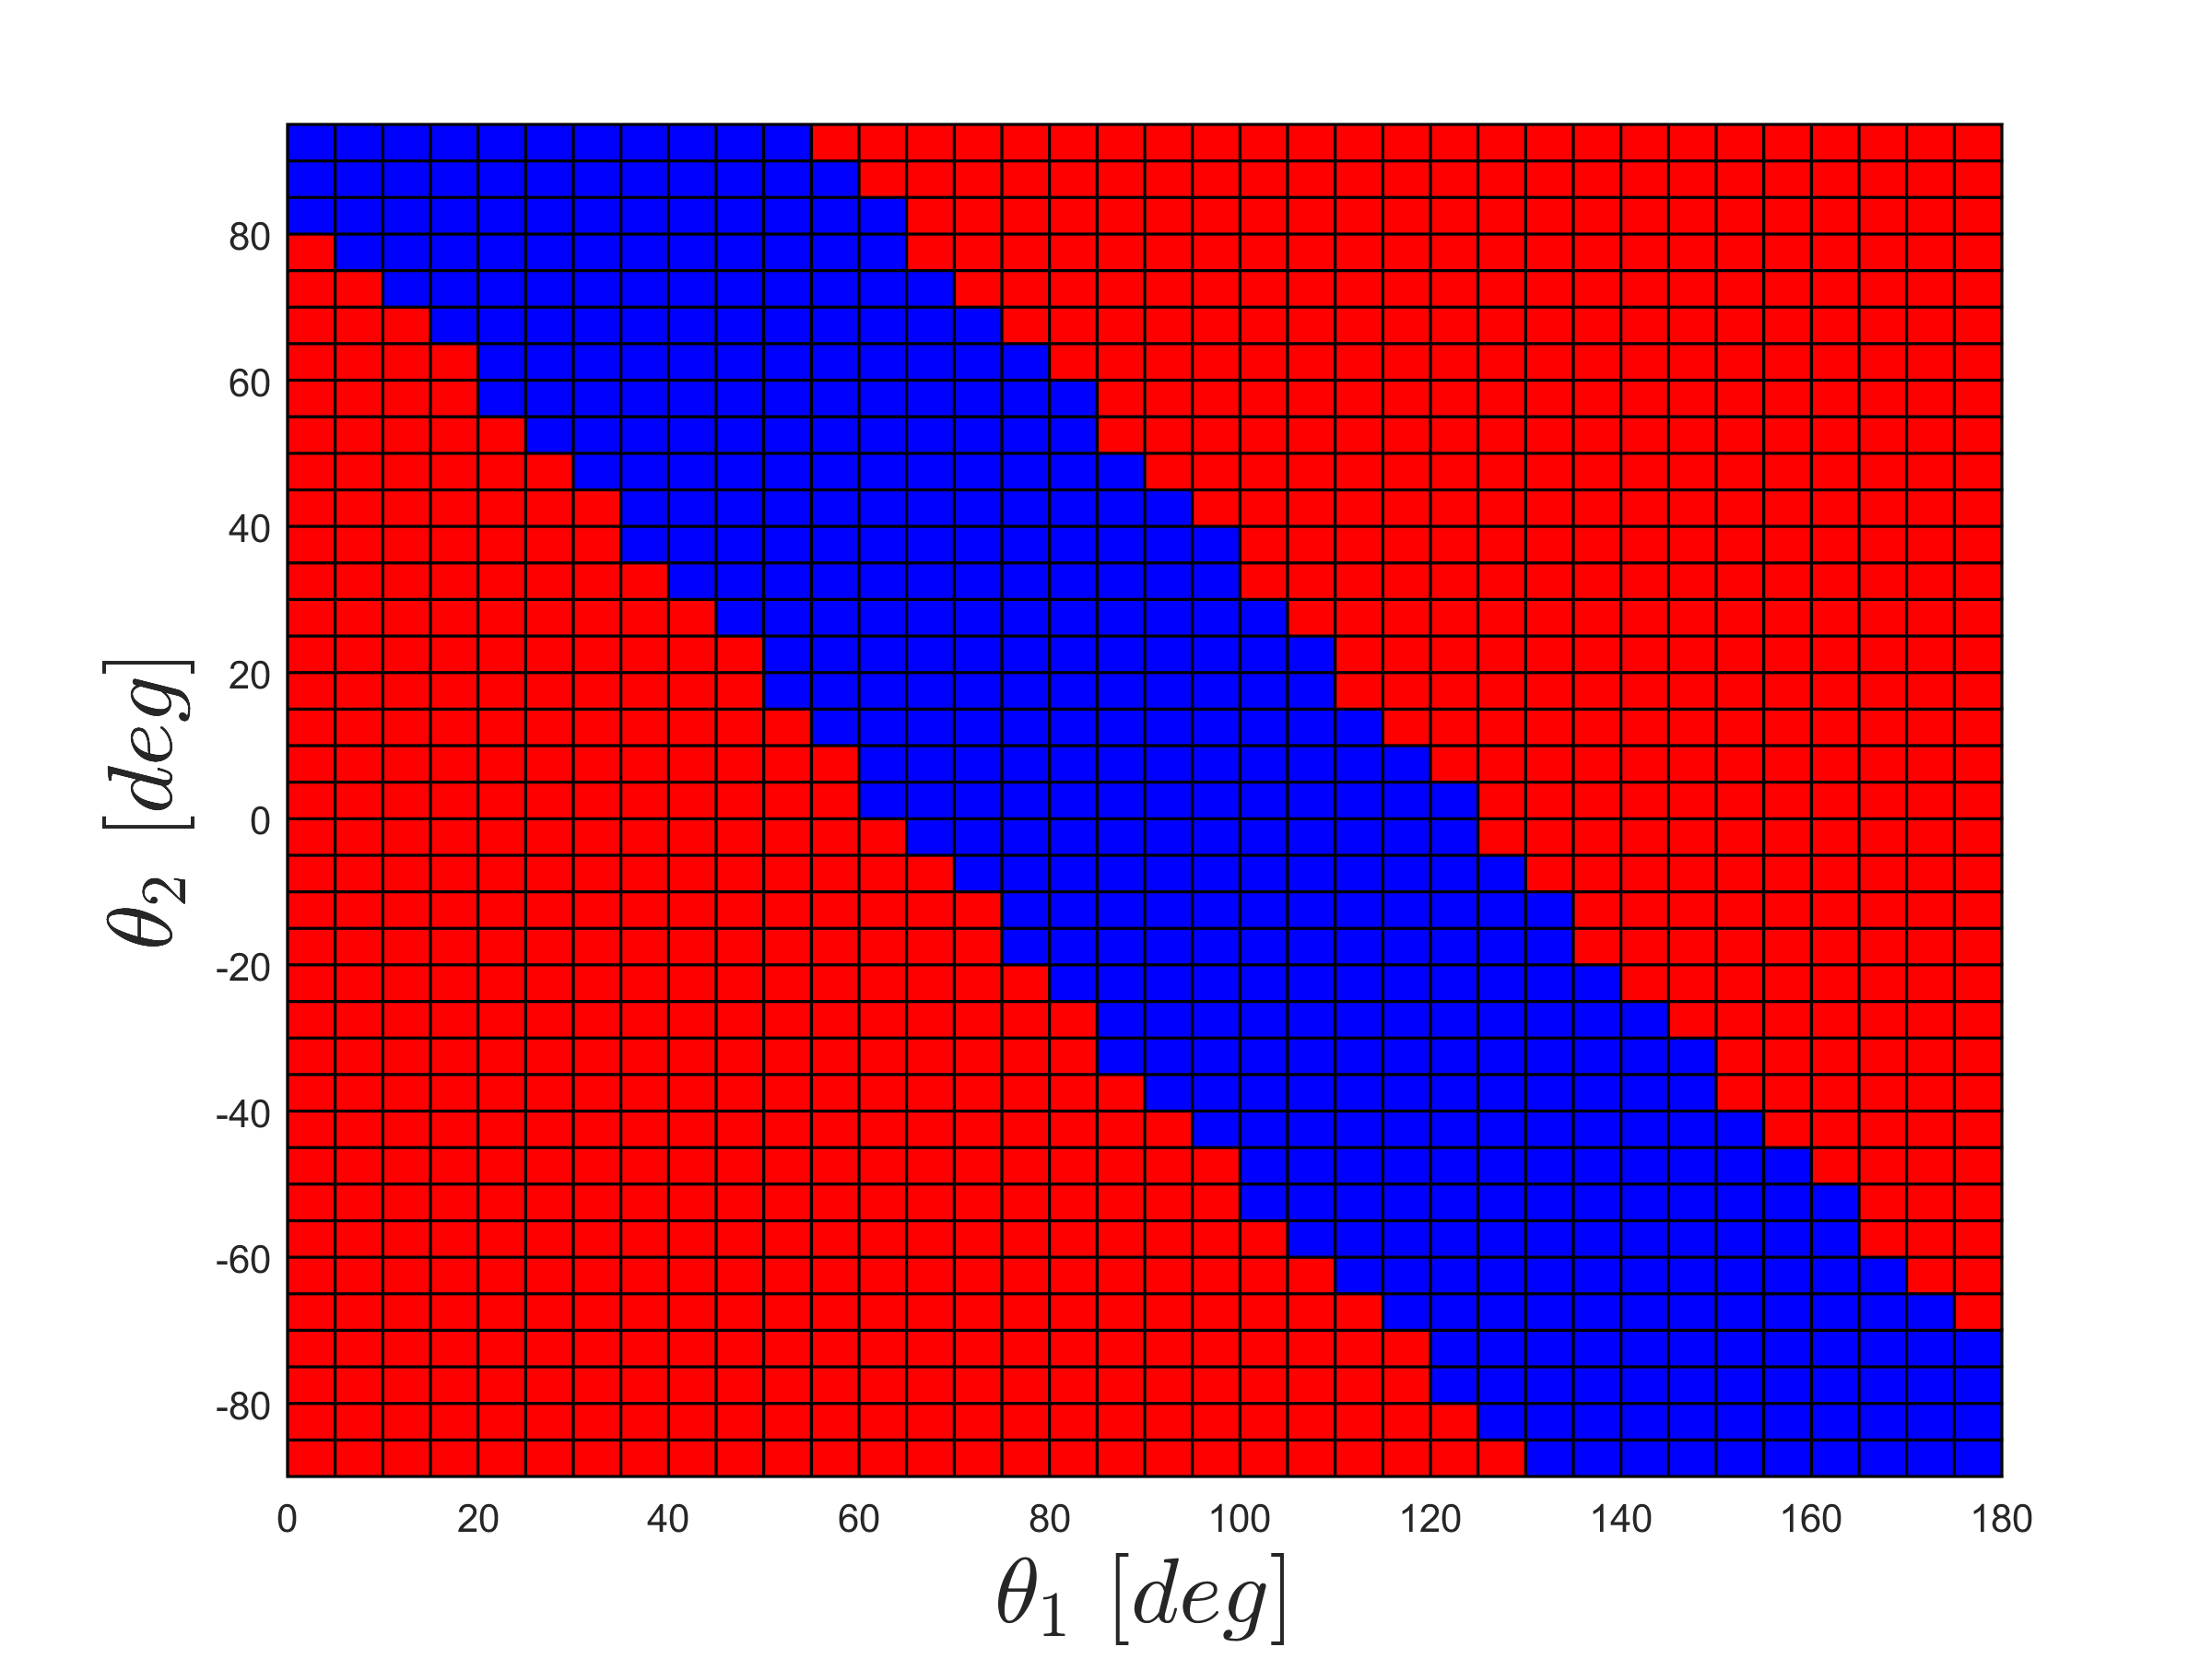
\includegraphics[width=0.85\linewidth]{img/RE_pendu_wykres_zbieznosci_bez_sat_lqr}
		\caption{Obszar zbieznosci dla samego sterownika liniowego}
		\label{fig:obszar_zbierznosci_tylko_liniowy}
	\end{figure}
	%
	Jako, �e oba sterowniki maj� inny obszar zbie�no�ci, postanowiono dokona� ich po��czenia w celu zwi�kszenia tego� obszaru, uzyskuj�c zale�no�� na sterowanie dan� wzorem 
	%
	\begin{equation}
	\label{eq:pendubot_u_hybrydowe}
	u = 
	\begin{cases}
	\frac{1}{L_g L_f^2 h} (-L_f^3 h + X), 
	& \text{for  }  
	\mathrm{something-} 1
	\\
	-K (x_r - x), 
	& \text{for  } 
	\mathrm{something-} 2
	\end{cases}
	\end{equation}
	%
	gdzie warunek prze��czenia dany jest zale�no�ci�....
	\\
	tutaj jakie� �adne wzorki opisujace te prze��czenie...
	\\
	W wyniku otrzymano obszar zbierzno�ci przedstwiony na Fig.~\ref{fig:obszar_zbierznosci_stero_hybrid_bez_saturacji}.
	%
	\begin{figure}[!ht]
		\centering
		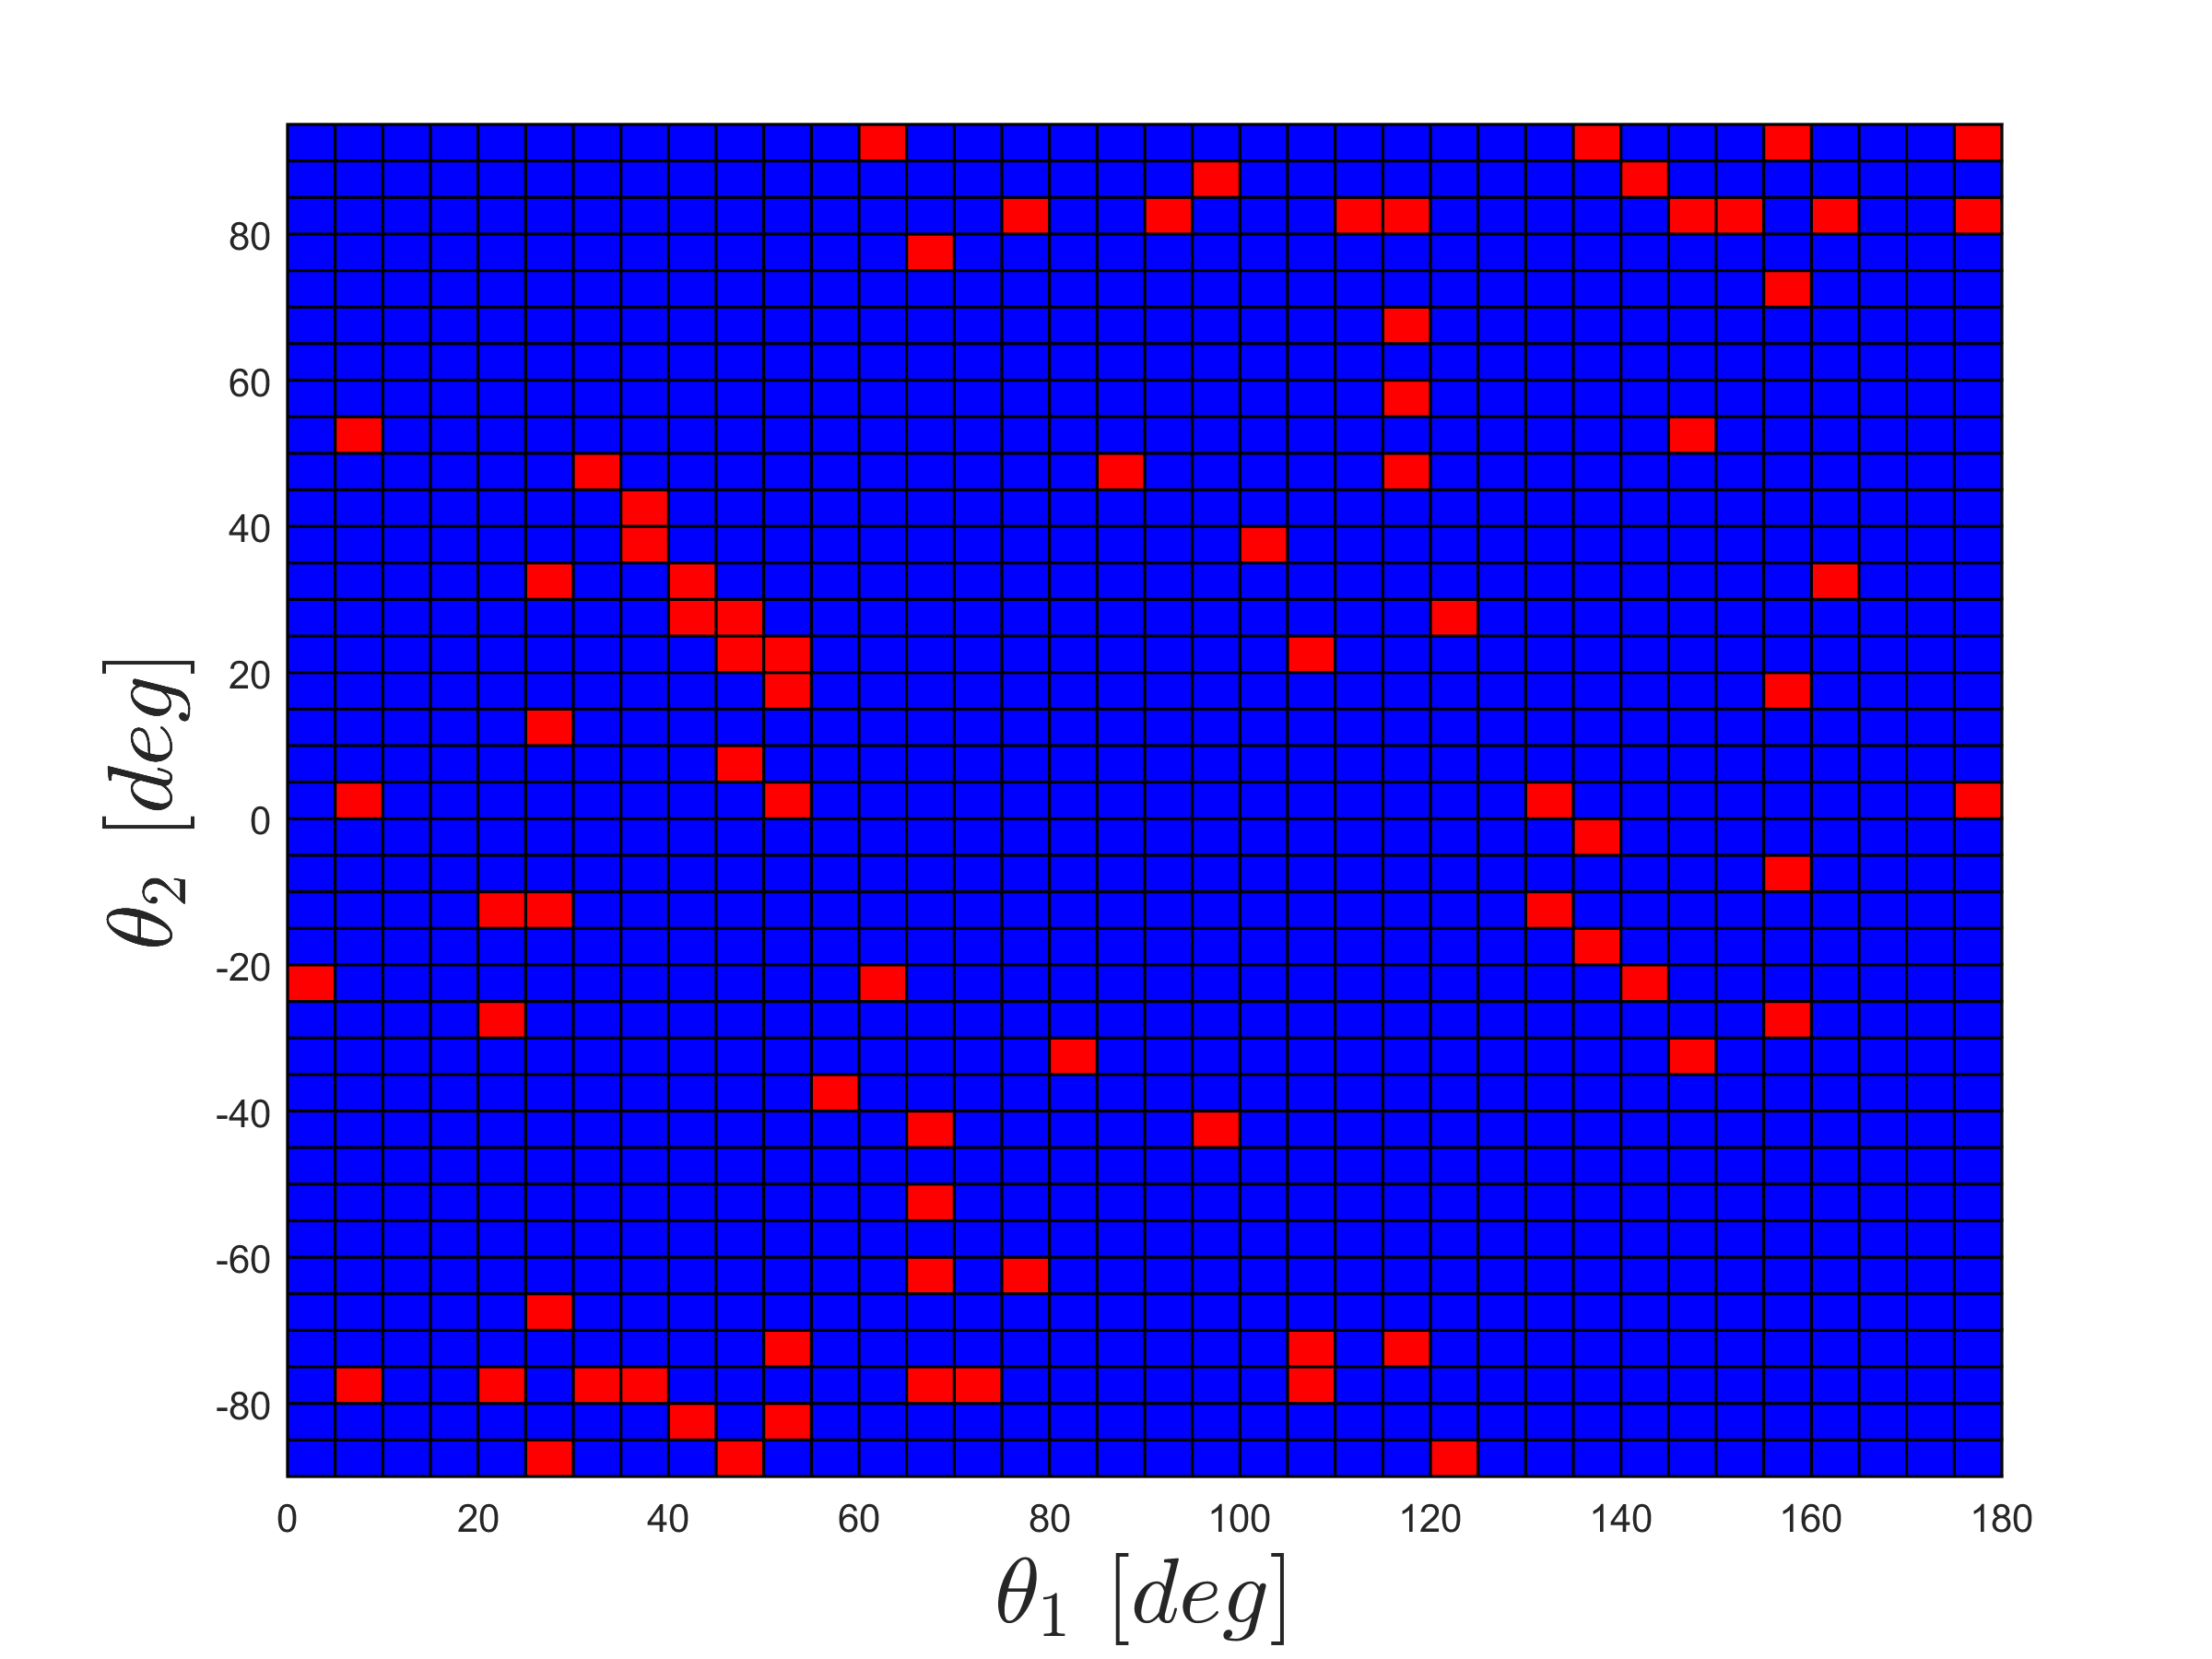
\includegraphics[width=0.85\linewidth]{img/RE_pendu_HYBRID_wykres_zbieznosci_bez_sat}
		\caption{Obszar zbieznosci dla sterownika hybrydowego -- bez saturacji}
		\label{fig:obszar_zbierznosci_stero_hybrid_bez_saturacji}
	\end{figure}
	%
	%
}
%In this article authors employ the LQR (\textit{Linear Quadratic Regulator}) controller to settle the robot at the equilibrium pose.
\\
%
%
As discussed above, the Pendubot control consists of two regulators.
The first one is a swing-up-like type, whose task is to bring the manipulator near the equilibrium point.
When the robot is in the error tunnel defined by the $\delta$  parameter, it switches to the LQR controller (as in \cite{grecki_lqr}).
This controller is designed to keep the system at an equilibrium pose.
It consists of a state-feedback part together with the $K$-gain vector.
Finally, the control rule for Pendubot can be written in the following form:
%
%
\begin{equation}
\label{eq:pendubot_u1}
u = 
\begin{cases}
\frac{1}{L_g L_f^2 h} (-L_f^3 h + X), 
& \text{for  }  
\gamma(\theta_2) < |\delta_d| 
\\
-K (x_r - x), 
& \text{for  } 
\gamma(\theta_2) > |\delta_d| 
\end{cases}
\end{equation}
%
%
%
%
and 
$x = [q_{1}\ v_{1}\ q_{2}\ v_{2}]^\top$ is the state vector 
a 
$x_r = [q_{r1}\ v_{r1}\ q_{r2}\ v_{r2}]^\top$ is the reference state vector, 
$\omega_0$ i $K = [k_1\ k_2\ k_3\ k_4]$ are controllers gains,
$\delta_d$ is a desired value of parameter $\delta$ from Eq~(\ref{eq:wektory_f_oraz_g}).





\subsection{Robot parameters}
\label{sec:parametry_robota}

The choice of the robot parameters (Table \ref{tab:parametry_robota}) in the simulation  was selected in order to adapt them to the physically existing mechanism, i.e. to the one-legged robot presented in Fig.~\ref{fig:sprzet}.
This one-legged mechanism can be studied as a double inverted pendulum.
Considered robot was built in the Institute of Automation and Robotics at  Poznan University of Technology, as a testbed for a four-legged walking robot presented in \cite{michalski_1_noga, parulski_michalski}.
%The robot parameters are collected in Table \ref{tab:parametry_robota}.
%
%
\begin{table}[!ht]
	\caption{Robot parameters}
	\label{tab:parametry_robota}
	\centering
	\begin{tabular}{|c|c|c|c|c|}
		\hline 
		Link & Mass & Centre of mass & Length & Inertia
		\\ 
		%\hline 
		&  [$\mathrm{kg}$] & [$\mathrm{m}$] & [$\mathrm{m}$] & [$\mathrm{kg\, m^2}$]
		\\ 
		\hline 
		1 & 1.593 & 0.074 & 0.15 & 0.0119
		\\ 
		\hline 
		2 & 0.405 & 0.134 & 0.295 & 0.0117
		\\ 
		\hline 
		
	\end{tabular} 
\end{table}
%
%
%
The physical model depicted in Fig.~\ref{fig:sprzet} is driven by Maxon's 200W EC-Powermax~30 brushless motors with planetary gearhead of $n=53$ reduction.
Such drives provides the maximum torque of approximately $6$~Nm.
This value is considered as a saturation of the control input.
% which defines an additional constraint imposed on the model.
%
%
\begin{figure}[!ht]
	\centering
	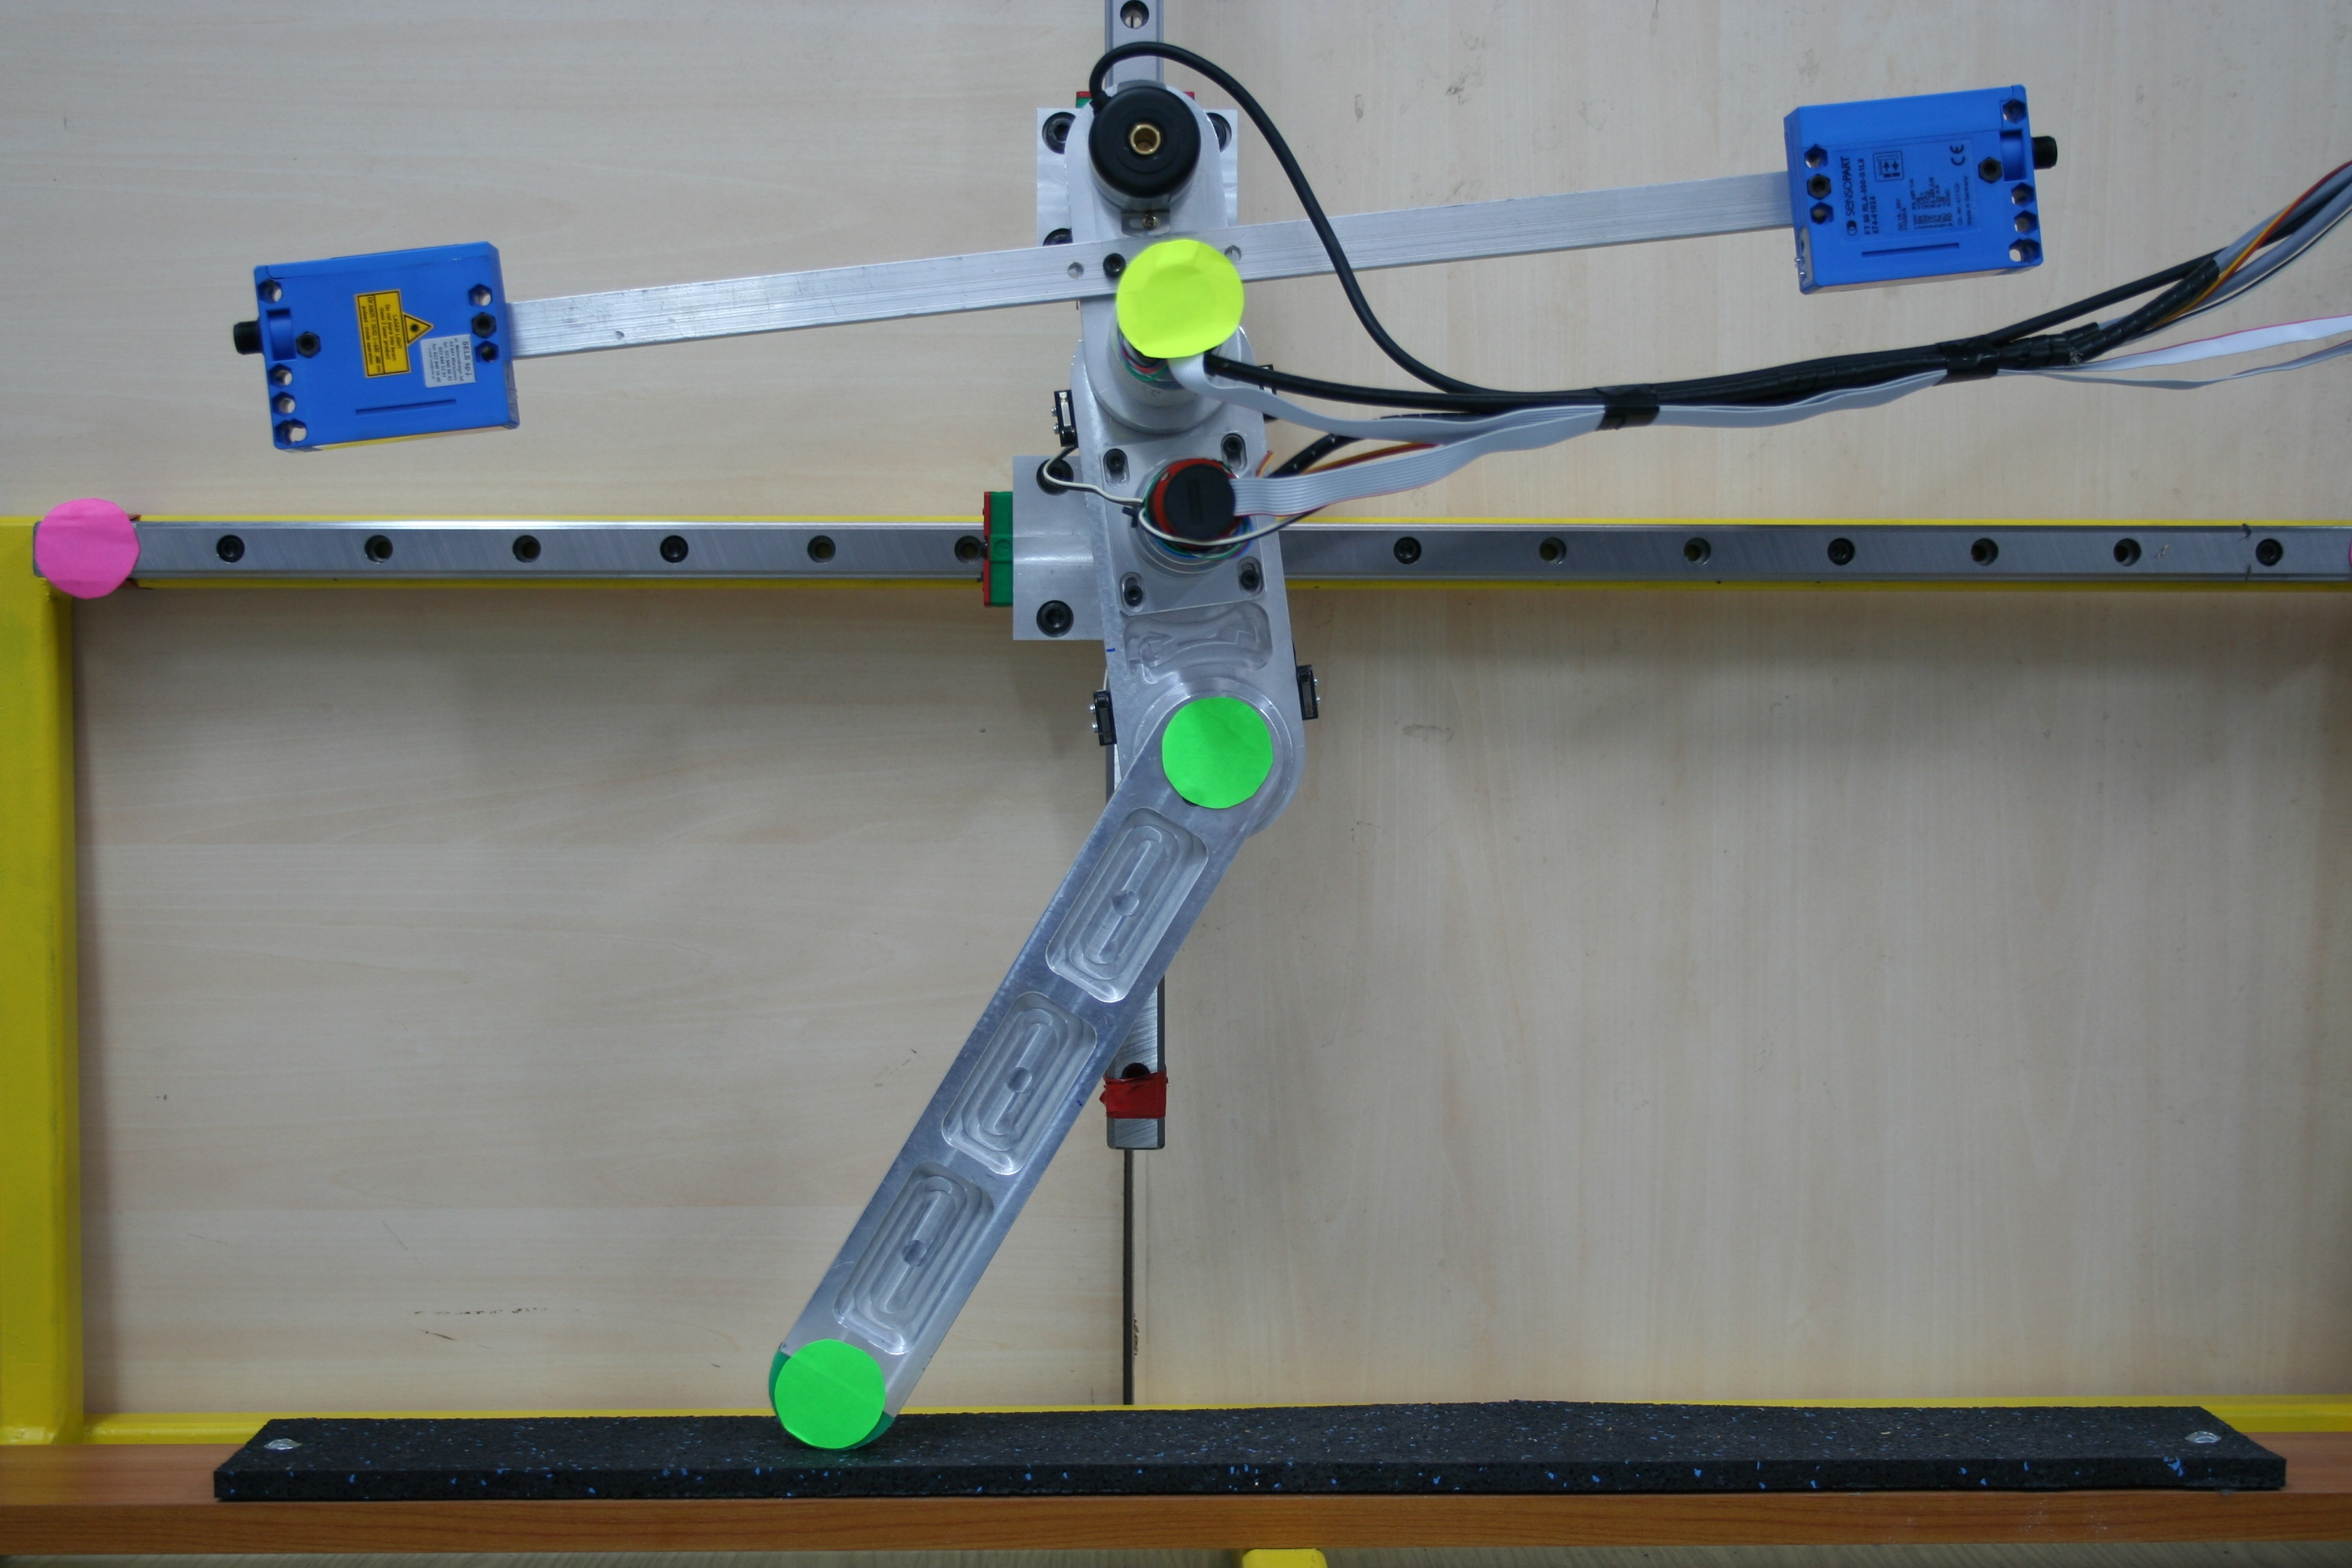
\includegraphics[width=0.85\linewidth]{img/sprzet}
	\caption{Experimental test-bed}
	\label{fig:sprzet}
\end{figure}





\subsubsection{Tuning the controllers parameters}



To acquire the best parameter  $\omega_0$, the integral of time-weighted absolute error (ITAE, Eq. (\ref{eq:ITAE})) performance index was used [\cite{tuning_itae}]
%
\begin{equation}
ITAE = \int_{0}^{\infty} t |e(t)| dt,
\label{eq:ITAE}
\end{equation}
%
where $t$ is  the  time  and $e(t)$ is  the  difference between reference value and controlled variable.
%
The best index value coincided with the $\omega_0 = 11$.
%
In the following step the $K$-vector was obtained, which is the LQR controller's gain.
In order to calculate them, the cost function $J$ (Eq.~\ref{eq:funkcja_J_lqr}), dependent on state and control signal, was defined.
%
%
%
\begin{equation}
J = \int_t^\infty \left(x^T Q x + u^T R u\right) d\tau,
\label{eq:funkcja_J_lqr}
\end{equation}
%
%gdzie Q, R s� macierzami wag dla ka�dego parametru.
where $Q$ and $R$ are the weight matrices for states and inputs, respectively.
The optimal $K$-gains ($K = [1, 520, 1050, 50]$) were obtained for the linear approximation of Eq.~(\ref{eq:wzor_2}) at the equilibrium point with $Q = 1000 I_{4\times 4}$ and $R = 0.5$.
%





% % % % % % % % % % % % % % % % % % % % % % % % % % % % % % % % % % %


\section{Simulation results}
\label{sec:symulacje_i_porowanie}




This section provides a simulation results of implementing control method (\ref{eq:pendubot_u1}) to the system in a form of (\ref{eq:dynamika_f_x_g}).
The aim of presented simulations was to stabilize the robot in upright position.
Authors also want to verify the convergence area of this new approach, which means that the set of initial conditions are going to be checked  to see whether they are appropriate to stabilize the robot under certain boundary conditions.
%
The algorithm verification is carried out in two ways.
Firstly, one wants to know how the algorithm behaves when no restrictions on the motor torque are imposed (Case I).
Secondly, the motor torque saturation is imposed on the model (Case II).
Thus, the algorithm is being checked whether is capable of controlling the model of physical robot.
%
To check how the algorithm behaves near the equilibirum pose, the system  (\ref{eq:dynamika_f_x_g})  with only LQR controller working was checked.
As a~result one obtained a~region of initial conditions (Fig.~\ref{fig:LQR_tunel_warunki}) that leads to upright position.
The plot of angular positions in links, ground reaction forces, decoupling matrix and motor torque are depicted in Fig.~(\ref{fig:LQR_pendu_th1th2_reakcja}, \ref{fig:LQR_pendu_mianownik_tau}).
Subsequently, the full controller (\ref{eq:pendubot_u1}) was used in order to verify considered control scheme.
%
%
\begin{figure}[!ht]
	\centering
	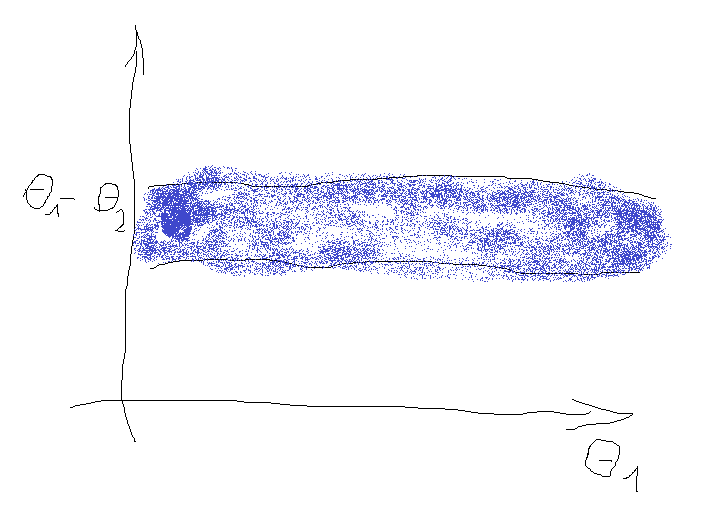
\includegraphics[width=0.85\linewidth]{img/LQR_sam}
	\caption{A~region of initial conditions (Fig.~\ref{fig:LQR_tunel_warunki}) that leads to upright position, for LQR controller.}
	\label{fig:LQR_tunel_warunki}
\end{figure}
%
%
%
\begin{figure}[!h]
	\centering
	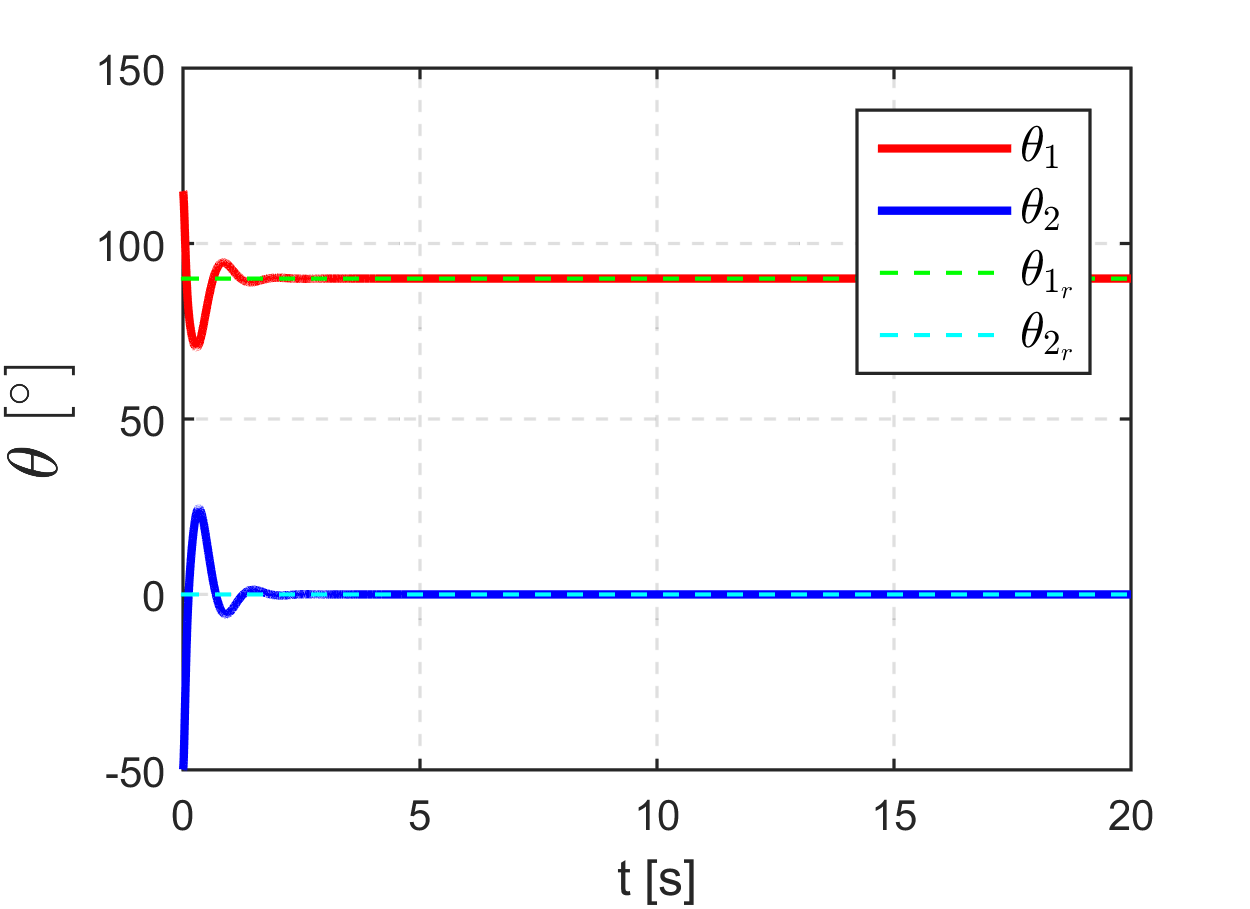
\includegraphics[width=0.49\linewidth]{img/pendubot_th1th2_z_lqr}
	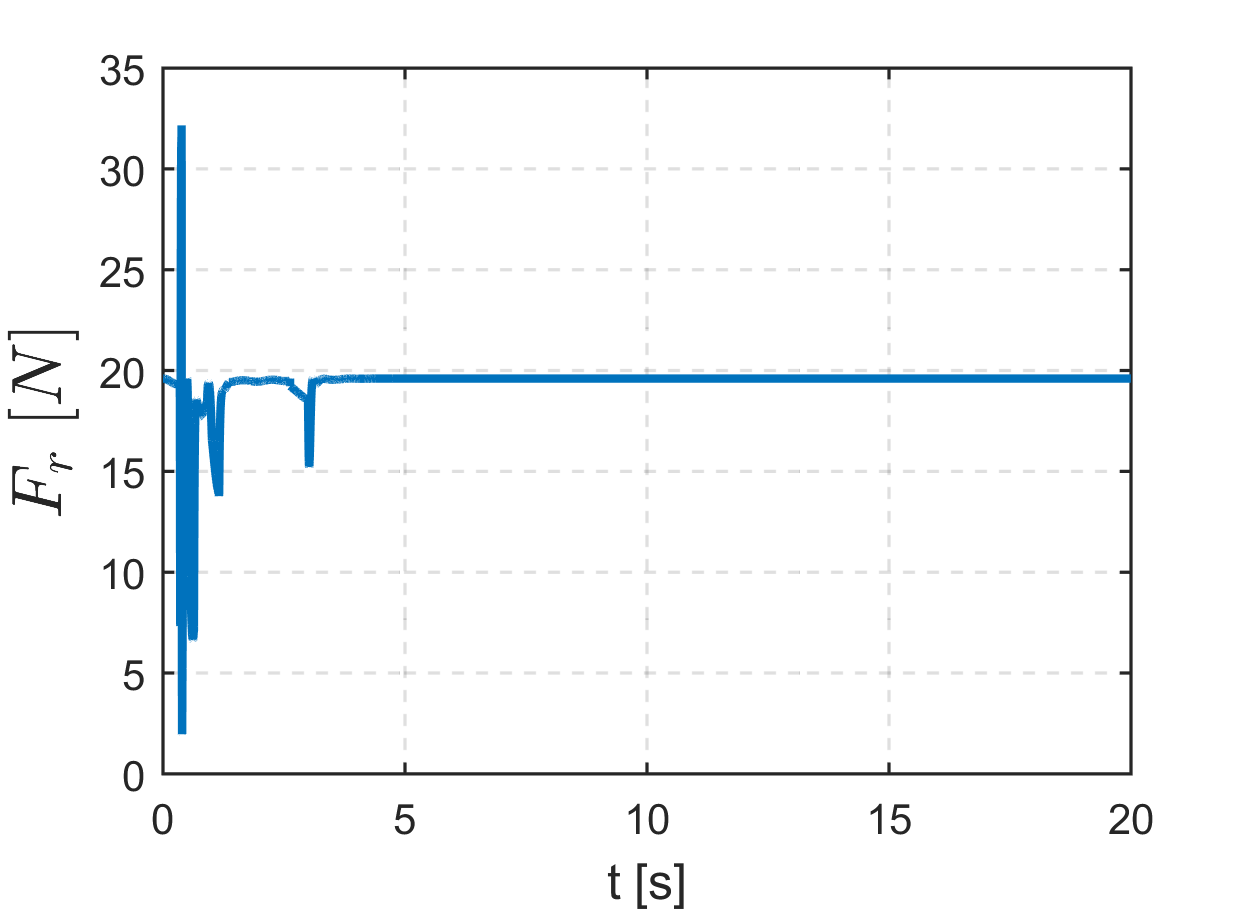
\includegraphics[width=0.49\linewidth]{img/Fr_bez_sat}
	\caption{The result of LQR controller -- a) Angular positions of links, b) Ground reaction forces}
	\label{fig:LQR_pendu_th1th2_reakcja}
\end{figure}
%
%
\begin{figure}[!h]
	\centering
	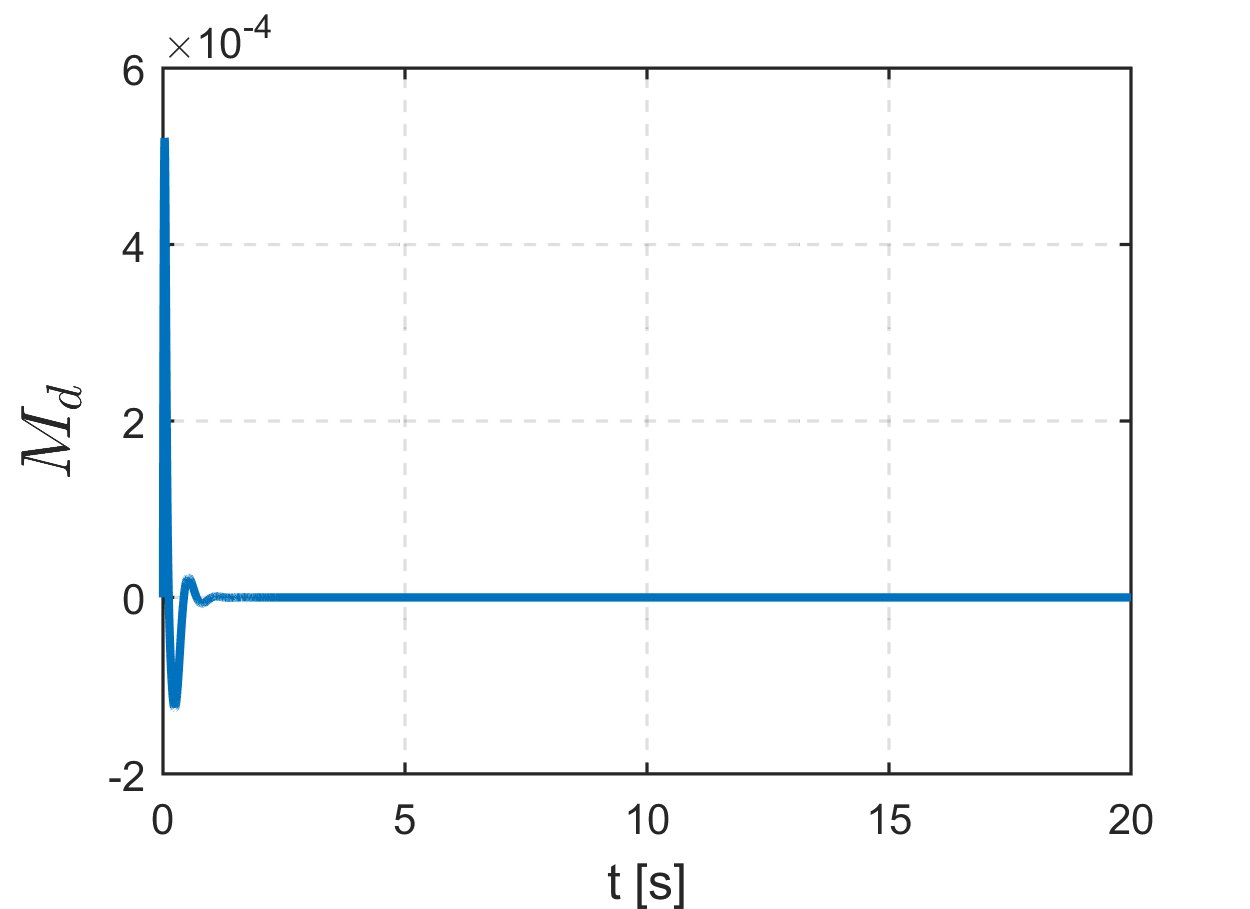
\includegraphics[width=0.49\linewidth]{img/M_d_z_lqr}
	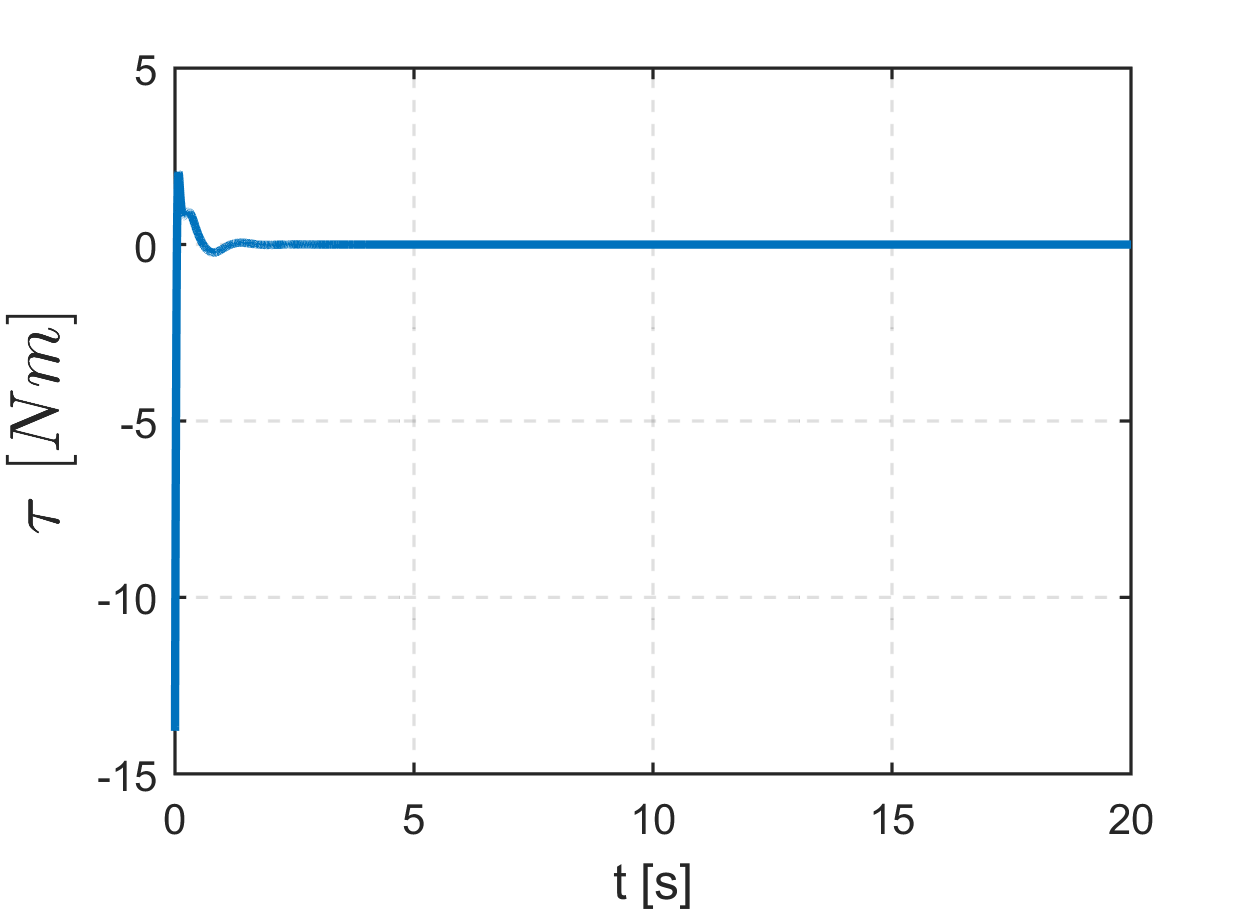
\includegraphics[width=0.49\linewidth]{img/tau_z_lqr}
	\caption{The result of LQR controller -- a) Decoupling matrix, b) Motor torque}
	\label{fig:LQR_pendu_mianownik_tau}
\end{figure}
% 
%%
%\begin{figure}[!ht]
%	\centering
%	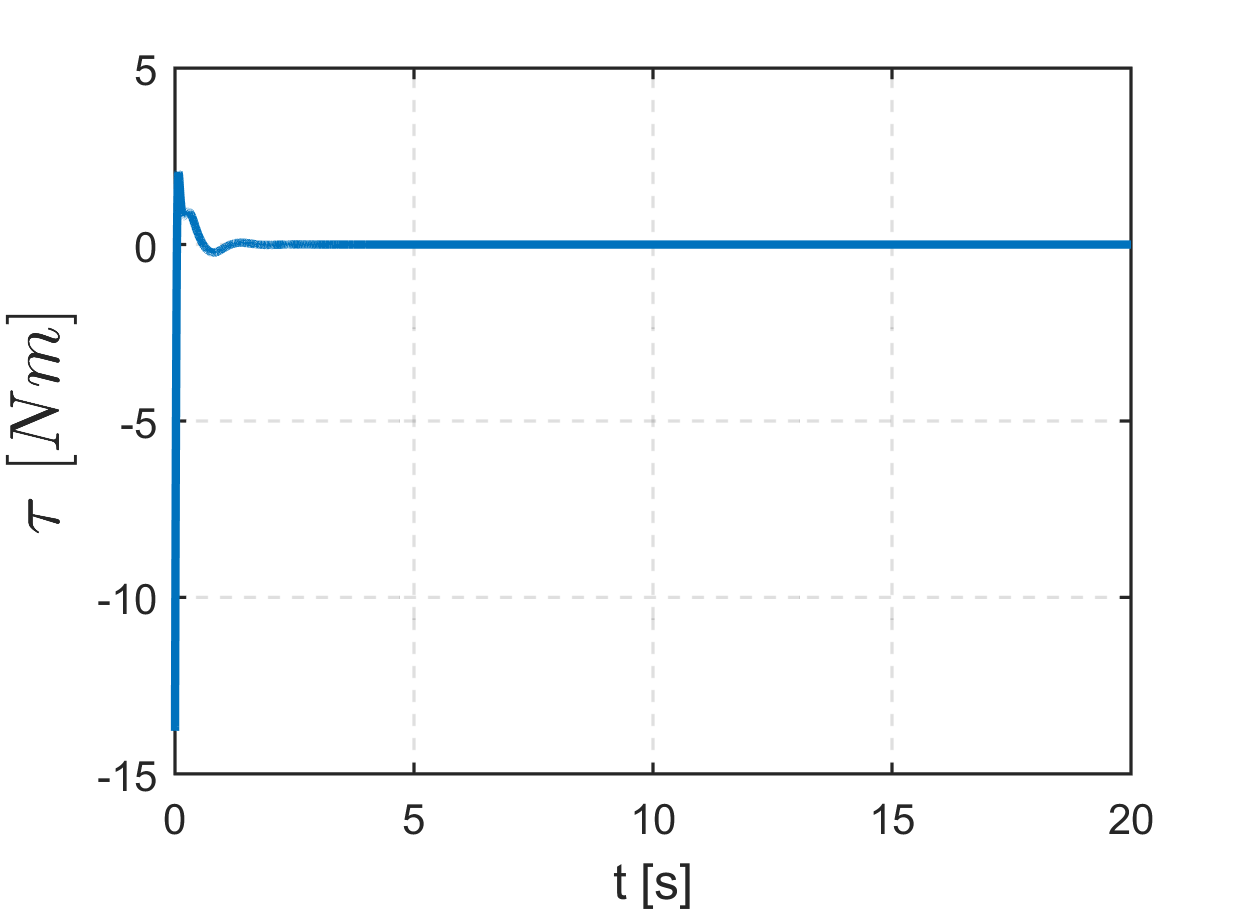
\includegraphics[width=0.49\linewidth]{img/tau_z_lqr}
%	\caption{Motor torque -- only LQR}
%	\label{fig:LQR_pendu_tau}
%\end{figure}
%
%
%\begin{figure}[!h]
%\centering
%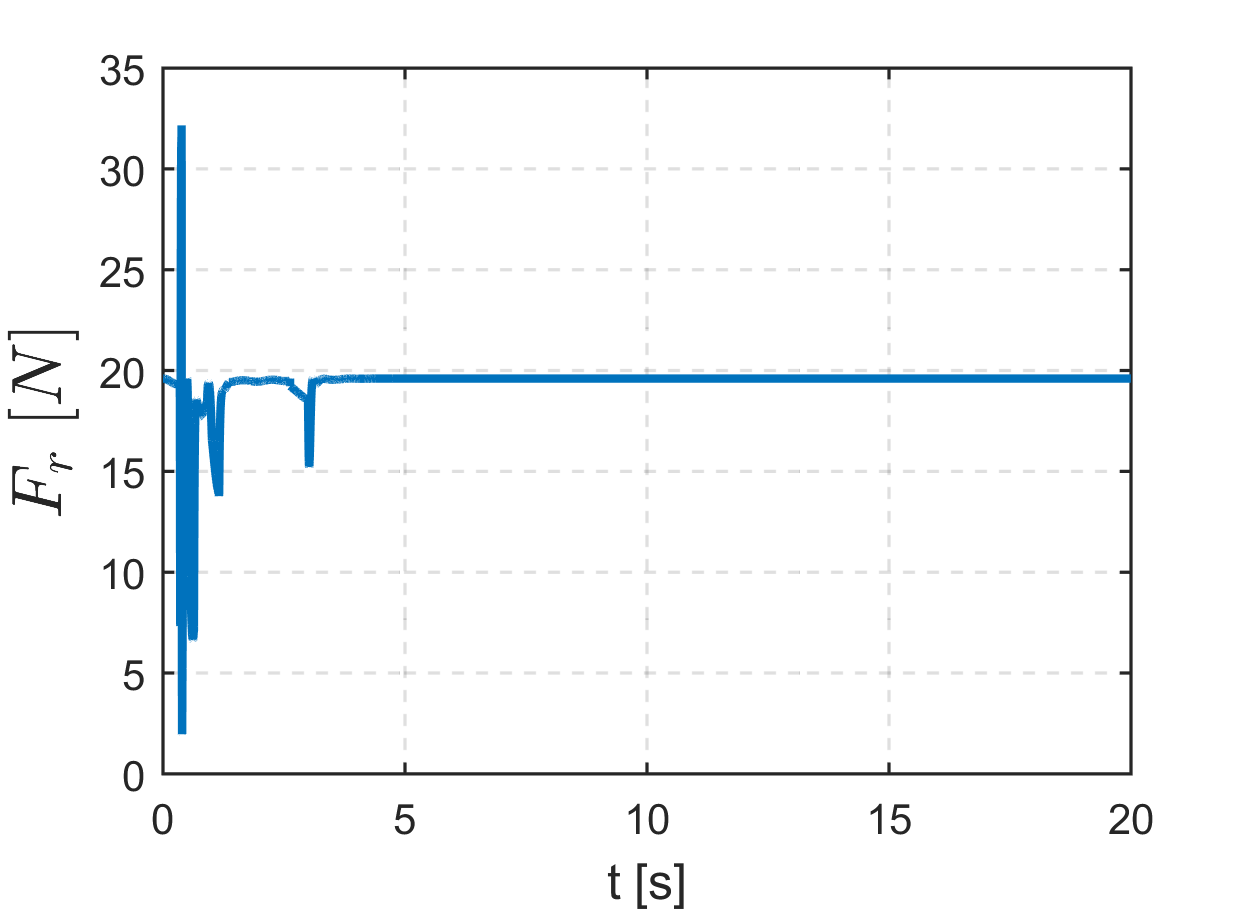
\includegraphics[width=0.9\linewidth]{img/Fr_bez_sat}
%\caption{Ground reaction forces -- only LQR}
%\label{fig:LQR_pendu_reakcja}
%\end{figure}
%
%
After applying the  controller (\ref{eq:pendubot_u1}) several conditions had to be imposed on the model.
One of them is a restricion imposed on initial angular velocities in the joints.
This situation is not favorable, as there is no any initial energy in the system at the beginning of the Pendubot movement.
The algorithm must provide a~great deal of energy to drive the robot from starting to desired position, and not to fall at the very beginning of the movement. 
Moreover, the robot is not fixed to the ground and the reaction forces are considered preventing the robot to liftoff.
%

The algorithm is not able to stabilize the Pendubot from any initial conditions, with the adopted assumptions.
It is interesting to see how far can the Pendubot be moved away from the equilibrium pose, to be stabilized in the upright position under certain boundary conditions.
The desired stabilization pose was the upright position for which the angles $\theta_{1r}$ and $\theta_{2r}$ were equal $\frac{\pi}{2}$ and $0$, respectively.
%
To determine the convergence area of analyzed method, a~series of tests were conducted.
%The results are depicted in Fig.~\ref{fig:re_pendu_wykreszbieznosci_case_1} for Case~I and  Fig.~\ref{fig:re_pendu_wykreszbieznosci_case_2} for second case.
%
The results are depicted in Fig.~\ref{fig:re_pendu_wykreszbieznosci_case_1} for the first case, where there is no saturation on the control signal.
The results depicted in Fig~\ref{fig:re_pendu_wykreszbieznosci_case_2} are for the case were motor torque is restricted to $6$~Nm, as in the section  \ref{sec:parametry_robota}.
%
The blue colour indicates the successful trial, while the red one indicates the initial conditions that lead to failure (robot collapse).
%
%
\begin{figure}[!ht]
\centering
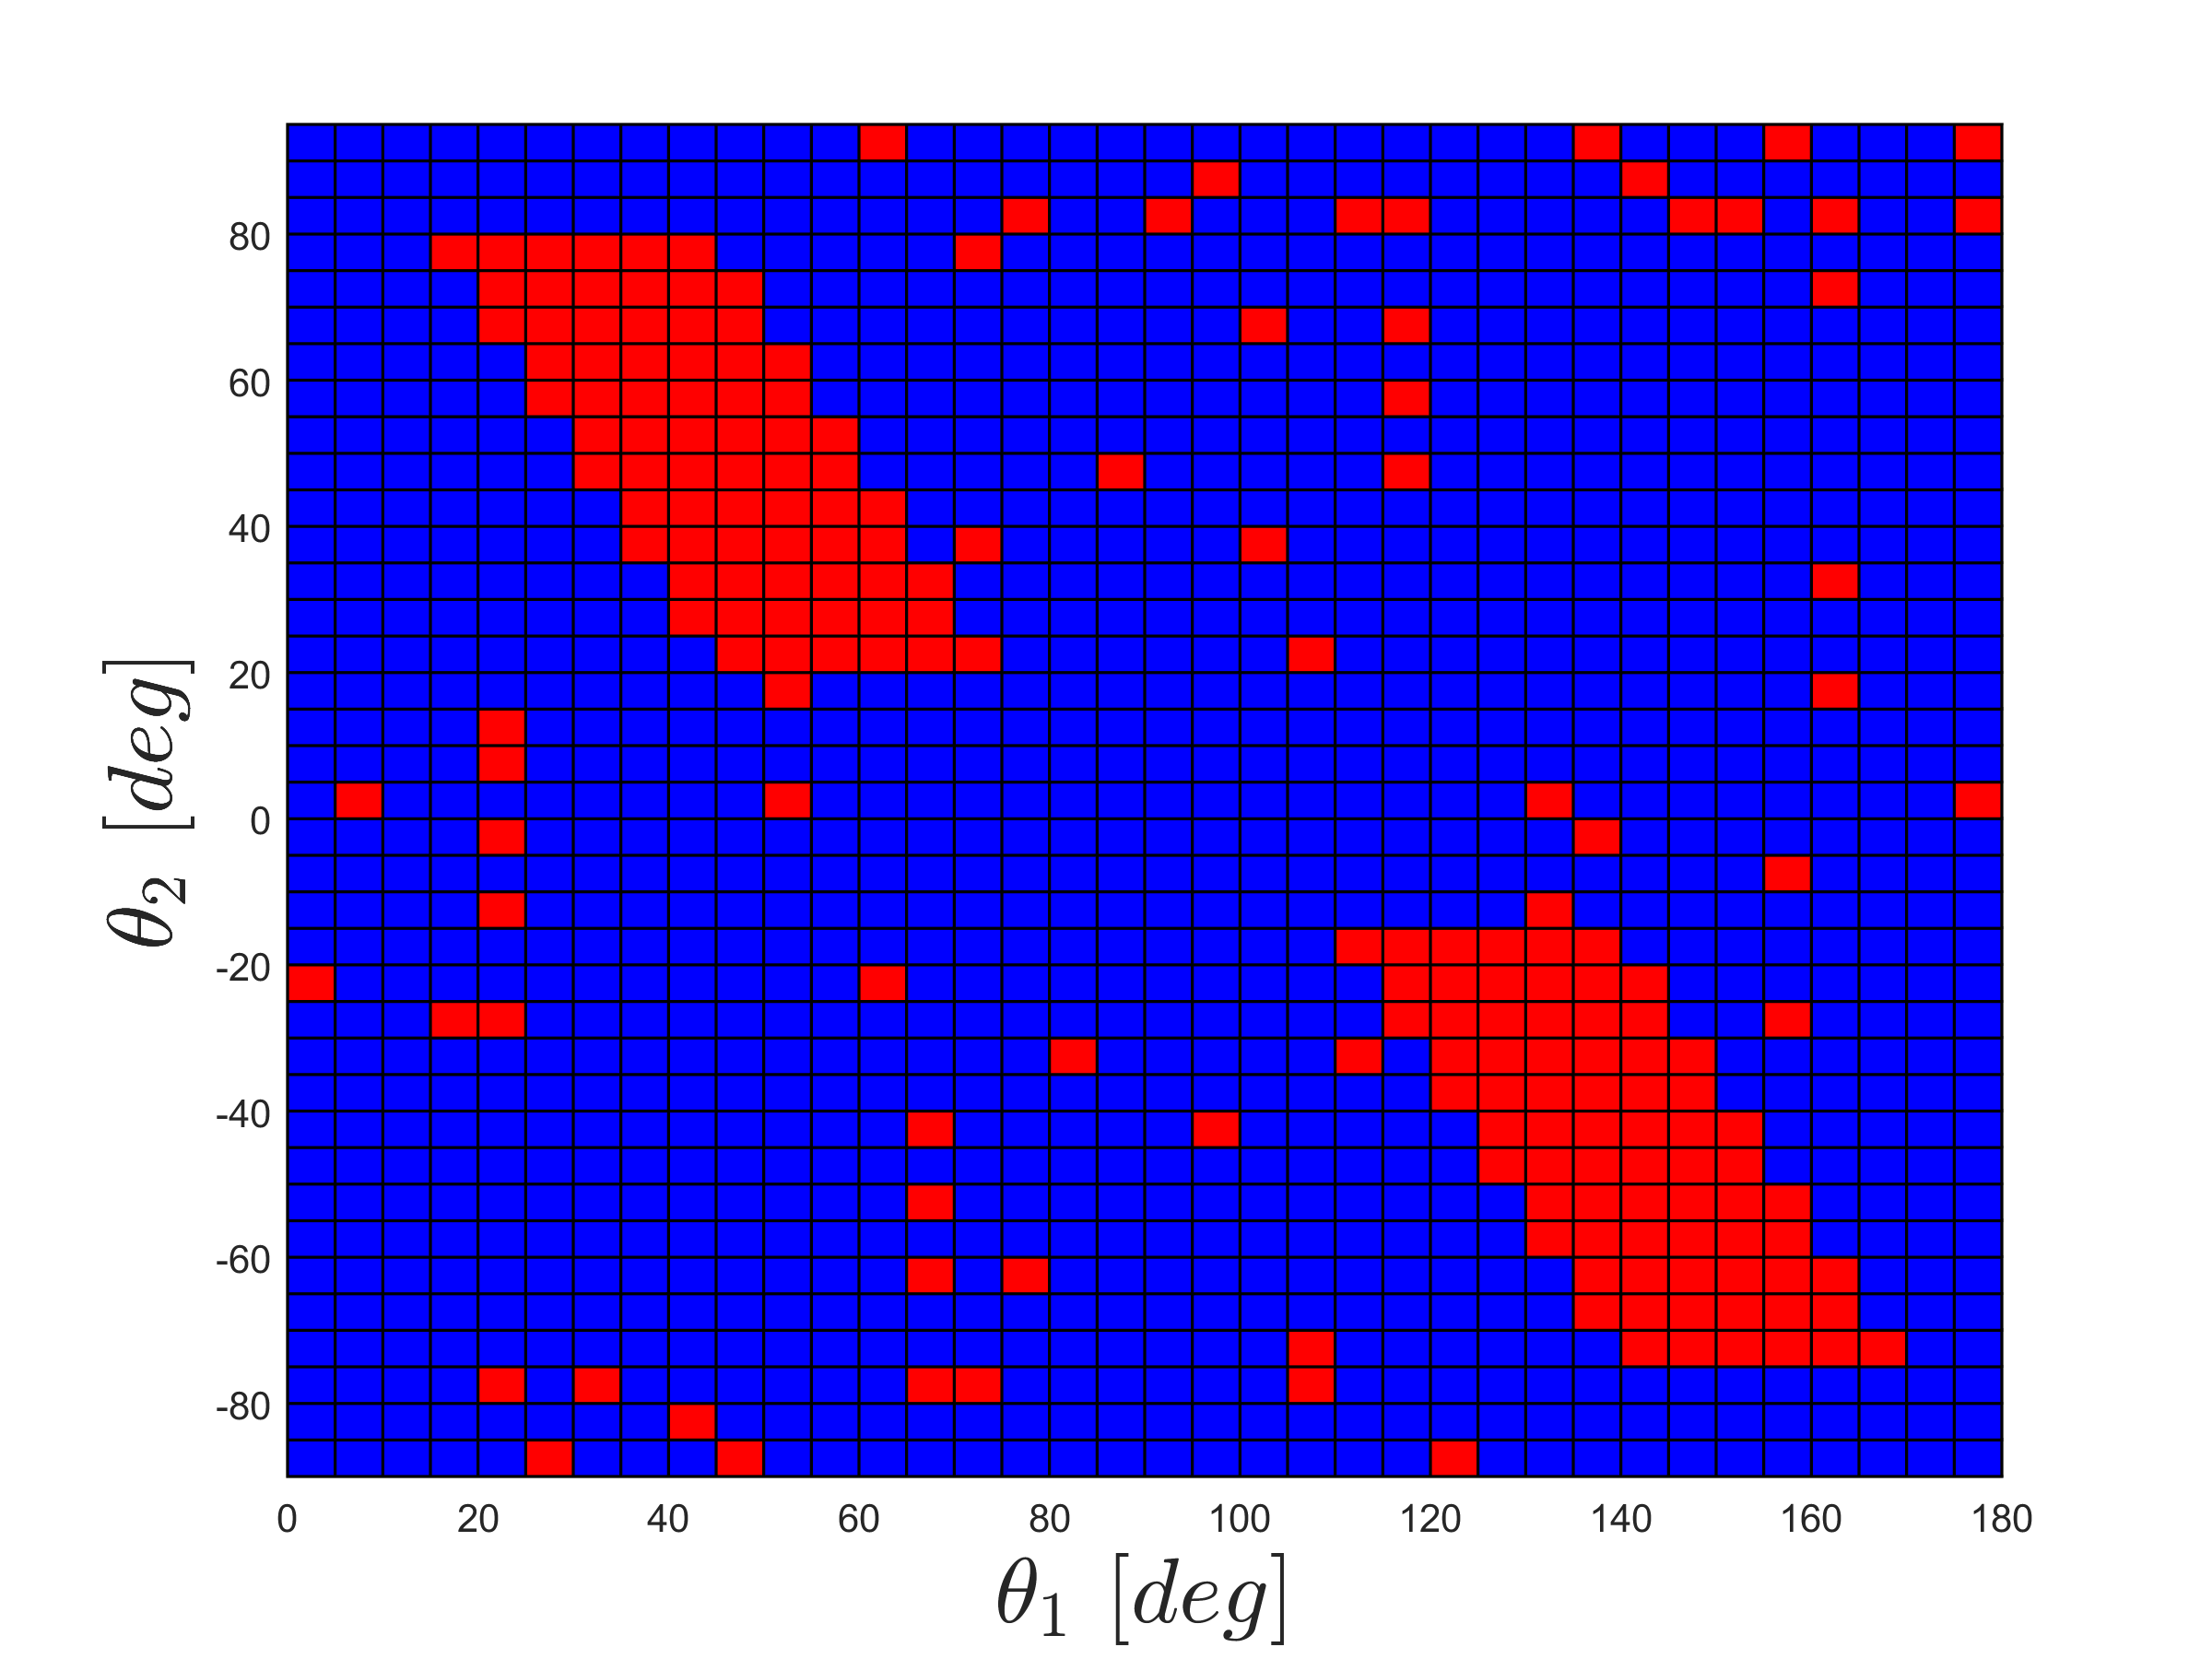
\includegraphics[width=0.85\linewidth]{img/RE_pendu_wykres_zbieznosci_bez_sat}
\caption{Convergence area -- Case I (blue  -- successful trial, red -- failure)}
\label{fig:re_pendu_wykreszbieznosci_case_1}
\end{figure}
%
%
\begin{figure}[!ht]
\centering
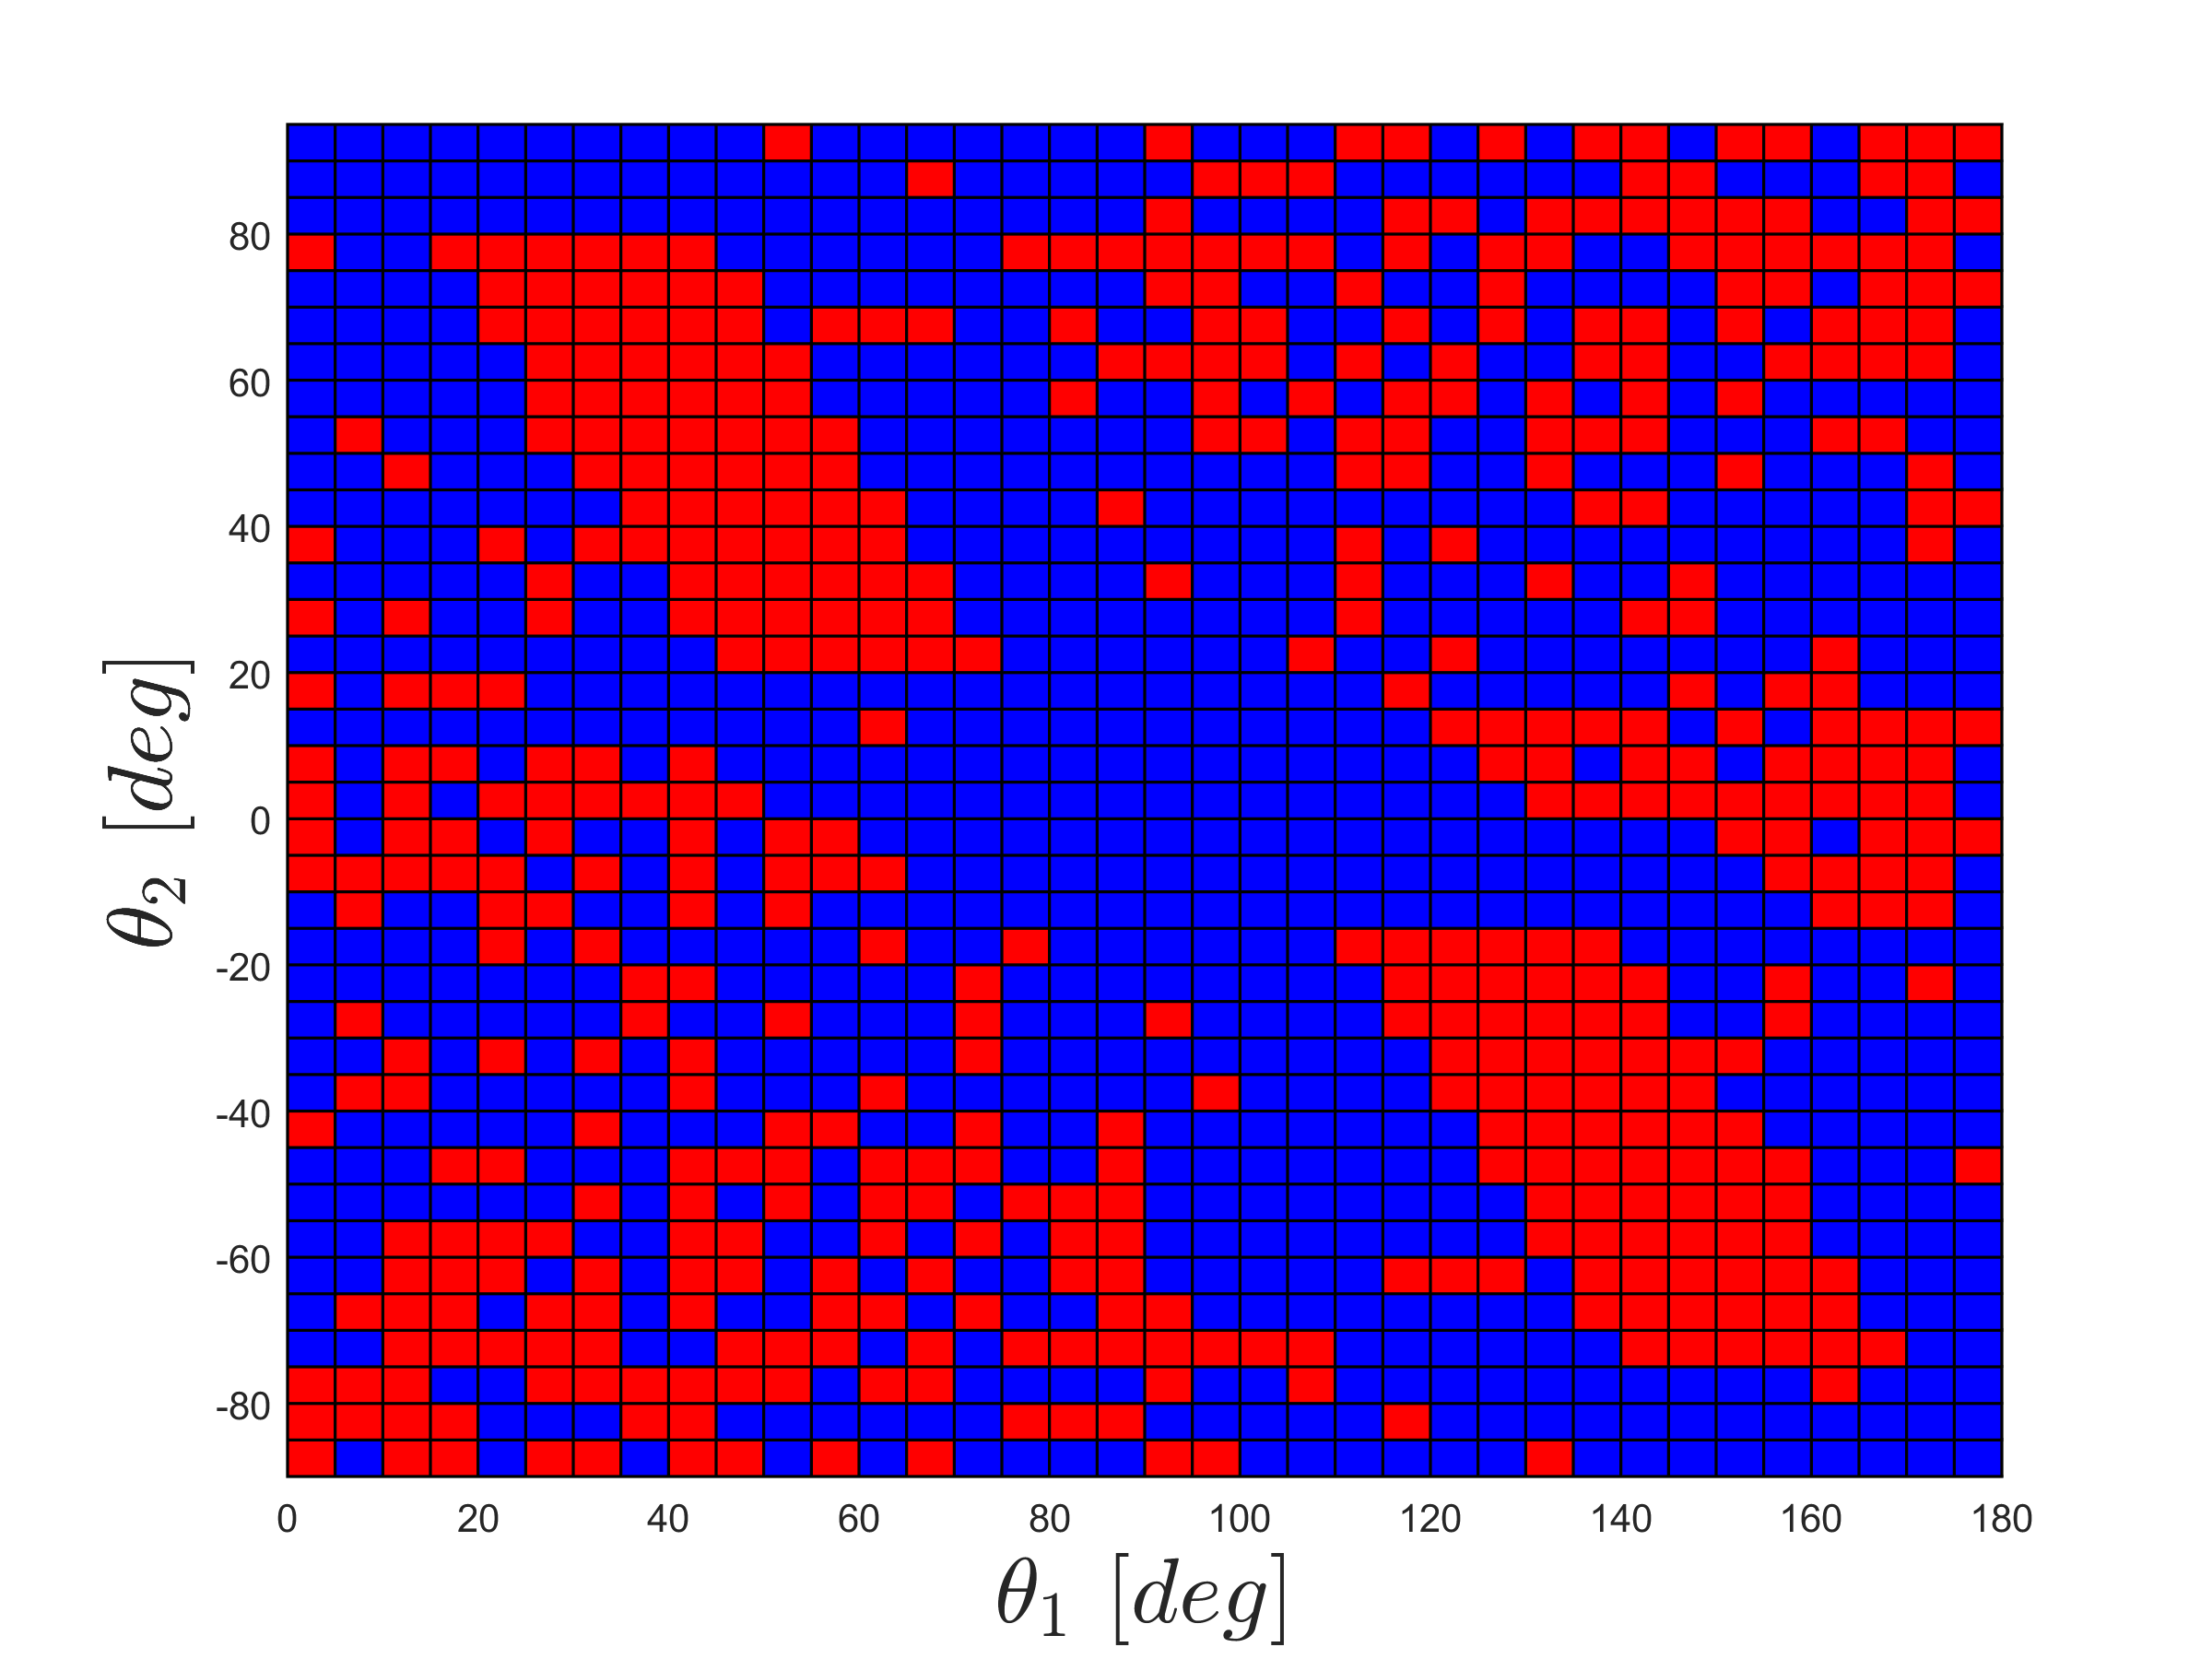
\includegraphics[width=0.85\linewidth]{img/RE_pendu_wykres_zbieznosci_sat}
\caption{Convergence area -- Case II}
\label{fig:re_pendu_wykreszbieznosci_case_2}
\end{figure}
%
%
Simulations in this paper were conducted with a step size equal 5$^\circ$, within range of $\theta_{1_0}$ from $0$ to $180^\circ$ and
$\theta_{2_0}$ from $-90^\circ$ to $90^\circ$, which gave more than 1300 simulation per approach.
These initial conditions mean that the swing-up problem is not considered, i.e. only situations where the robot is above the ground are taken into account.
The trial was being taken as successful while the error between actual and desired angle was smaller than  $\frac{1}{180}\pi \,$rad within simulation time  {\color{red} $t = 15 \,$s}. 
%

Considered algorithm does not guarantee that the robot will not reach singularity.
Thus, other constrains had to be imposed on the model.
%Thus, time must be another constraint imposed on the simulation.
As the time can be treated as the simulation time and a real time of executing the program, one should distinguish them.
First of them is a "standard" simulation time, calculated by solver.
The other one is the time of program's execution (or iterations of the program, to become independent of the computer's CPU).
The need of imposing such a constraint results from the nature of considered system.
Double inverted pendulum can reach a singularity position, which leads to discontinuities in some characteristics.
These causes that the solver and simulation "hangs" or crash.
%
Authors concluded that while {\color{black} 50000 iterations} of the program's execution no result was obtained (achieving the desired configuration), such a situation should be treated as the occurrence of singularities in the object and a crash of the program. 
\\
As mentioned before in section \ref{sec:respondek} the control signal explodes around equilibria.
Thus, the additional imposed restriction is the maximal value of $\sigma$ parameter from Eq.~(\ref{eq:pendubot_u1}).
Authors assume the $\sigma$ parameter as $\sigma = 0.04$, which was obtained by trail end error.
\\
The additional problem with execution the algorithm is the need of inverting the decoupling matrix $L_g L_f^2 h$ in Eq.~(\ref{eq:RE_acrobot_u}).
Fig.~\ref{fig:re_pendu_mianownik} depicts a plot of $L_g L_f^2 h$ during one exemplary simulation trial, for Case~I and II, respectively.
To overcome the problem of inverting this matrix, authors use an arbitrarily chosen parameter $\epsilon$, which was added to $L_g L_f^2 h$  when was close to $0$.
Parameter $\epsilon$ can enlarge the region of attraction of analysed algorithm, but was not designed by \cite{Respondek_2019}.
This procedure can be treated as an attempt to improve  the performance of the algorithm.
The invertibility of $L_g L_f^2 h$ was another constraint imposed on the model.
%
\begin{figure}[!h]
	\centering
{\footnotesize a)}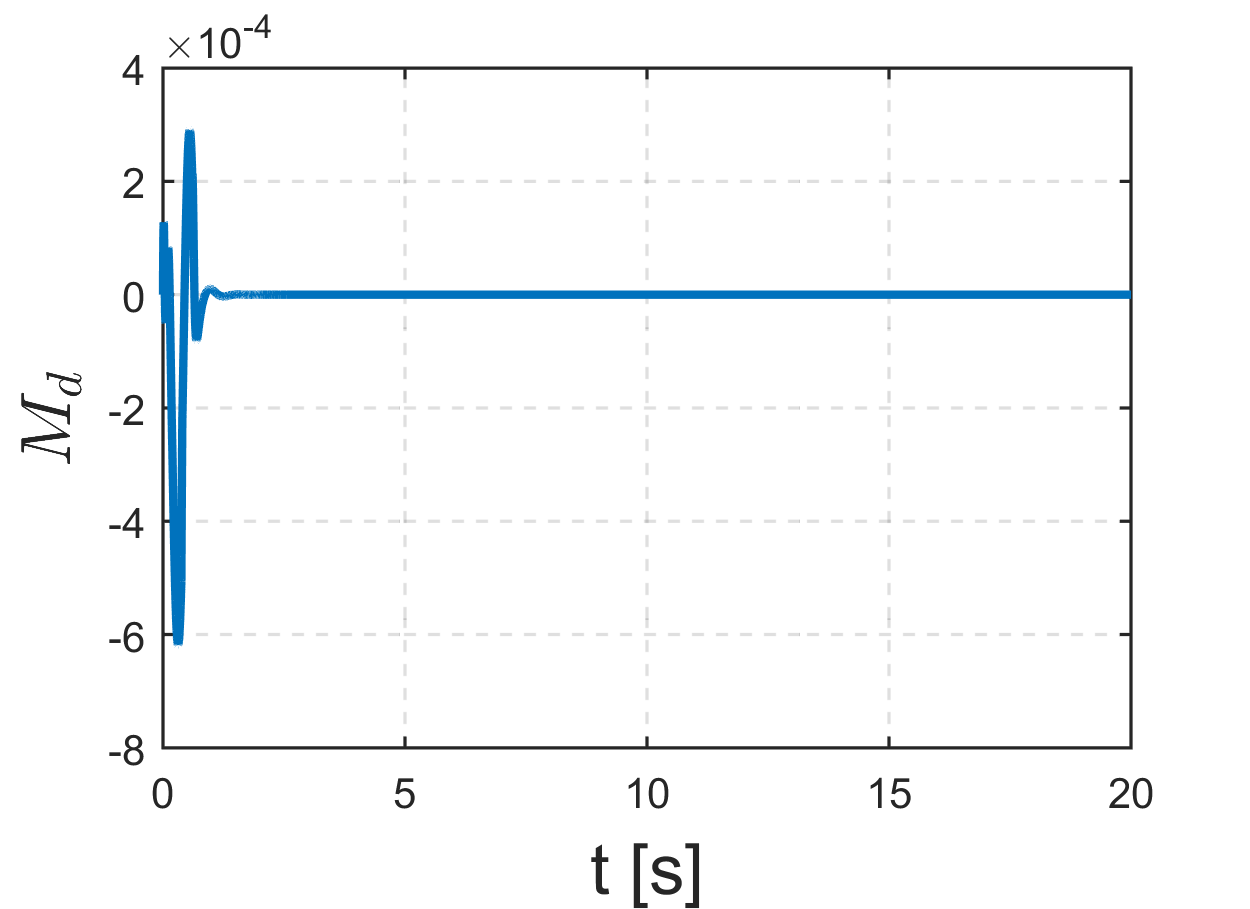
\includegraphics[width=0.46\linewidth]{img/M_d_bez_sat}
{\footnotesize b)}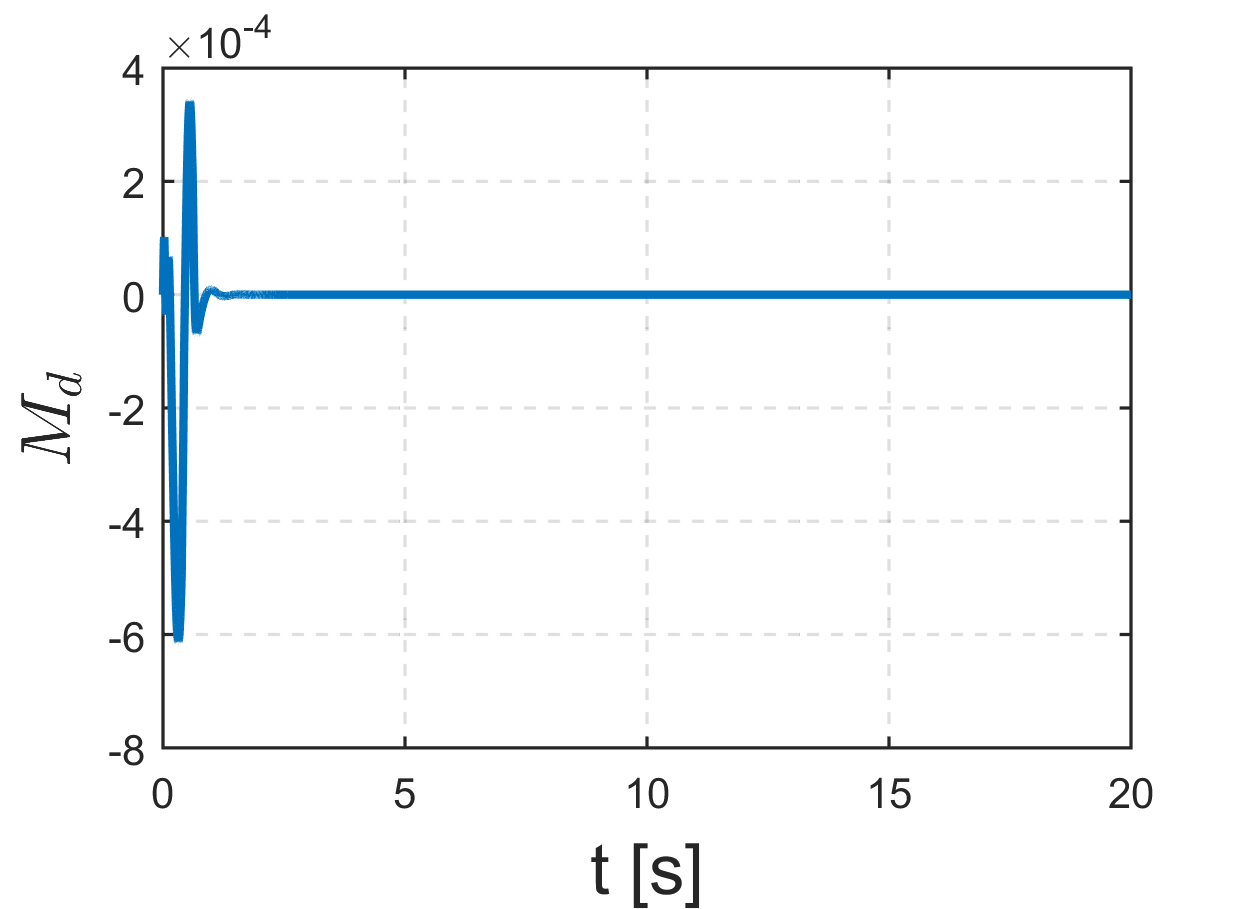
\includegraphics[width=0.46\linewidth]{img/M_d_z_sat}
\caption{Decoupling matrix -- a) Case I, b) Case II }
	\label{fig:re_pendu_mianownik}
\end{figure}
% 
%%
%\begin{figure}[!h]
%	\centering
%	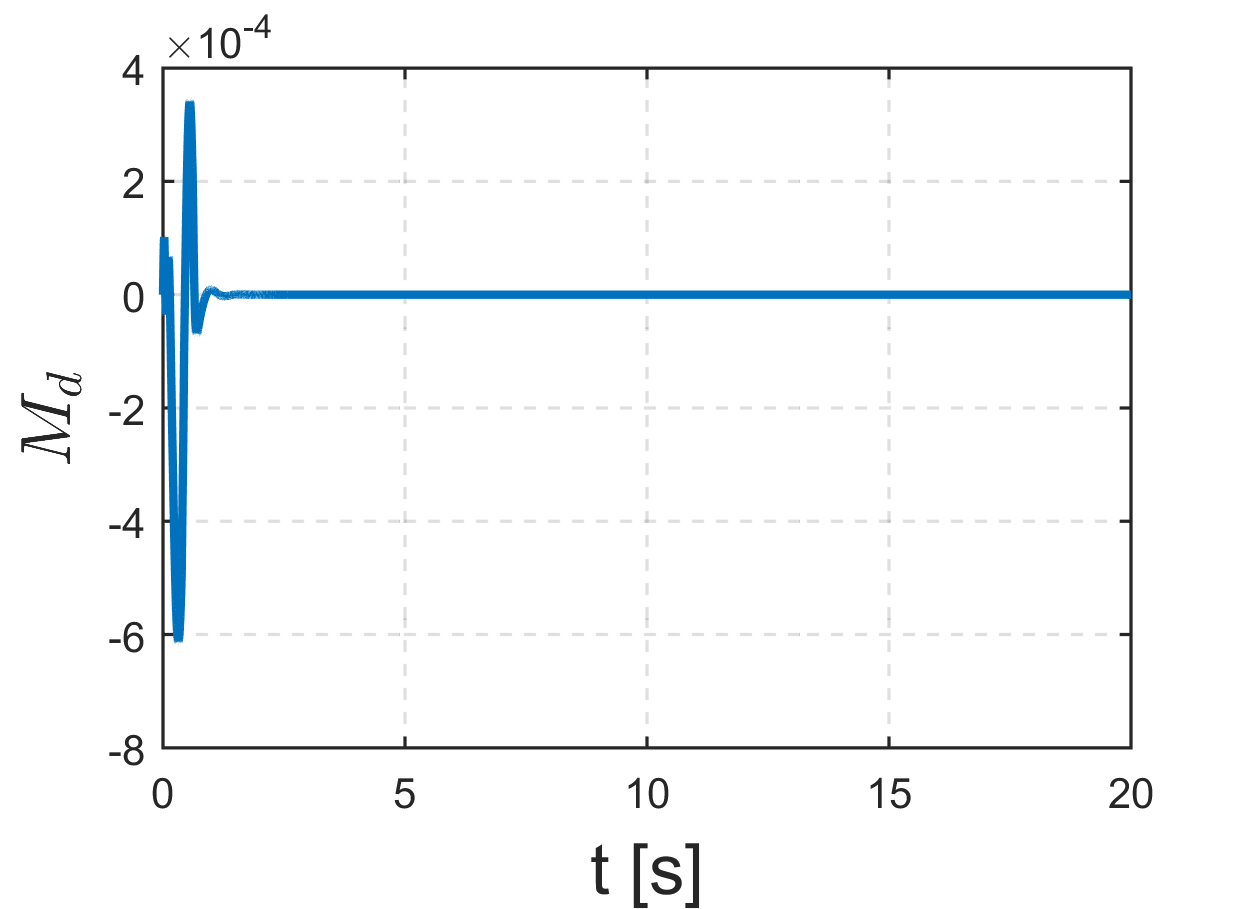
\includegraphics[width=0.85\linewidth]{img/M_d_z_sat}
%	\caption{Decoupling matrix -- Case II }
%	\label{fig:re_pendu_mianownik_case_2}
%\end{figure}
%% 






To see how the algorithm drives the robot to the reference upright position one of the successful trails from Fig.~\ref{fig:re_pendu_wykreszbieznosci_case_1} and Fig.~\ref{fig:re_pendu_wykreszbieznosci_case_2}  was chosen.
The common exemplary successful initial condition (for Case~I and II) was chosen as {\color{black} $\theta_{1_0} = 115^\circ$ and $\theta_{2_0} = -50^\circ$}.
%
The obtained angular trajectories are shown in Fig.~\ref{fig:re_pendu_th1th2_case_1} and Fig.~\ref{fig:re_pendu_th1th2_case_2} for the first and second Case, respectively.
%
%
\begin{figure}[!h]
	\centering
	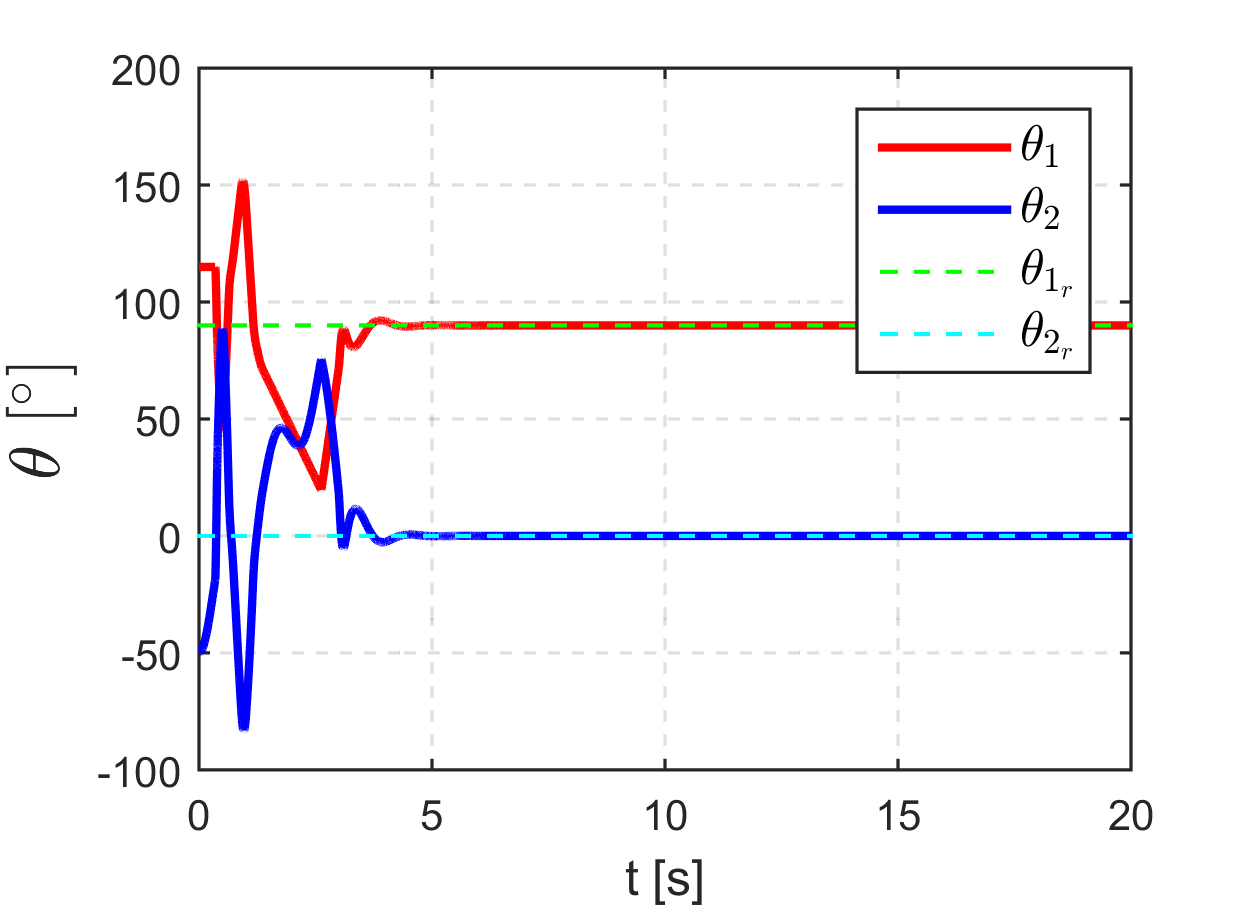
\includegraphics[width=0.85\linewidth]{img/pendubot_th1th2_bez_sat}
	\caption{Angular positions of links -- Case I}
	\label{fig:re_pendu_th1th2_case_1}
\end{figure}
%
%
\begin{figure}[!h]
	\centering
	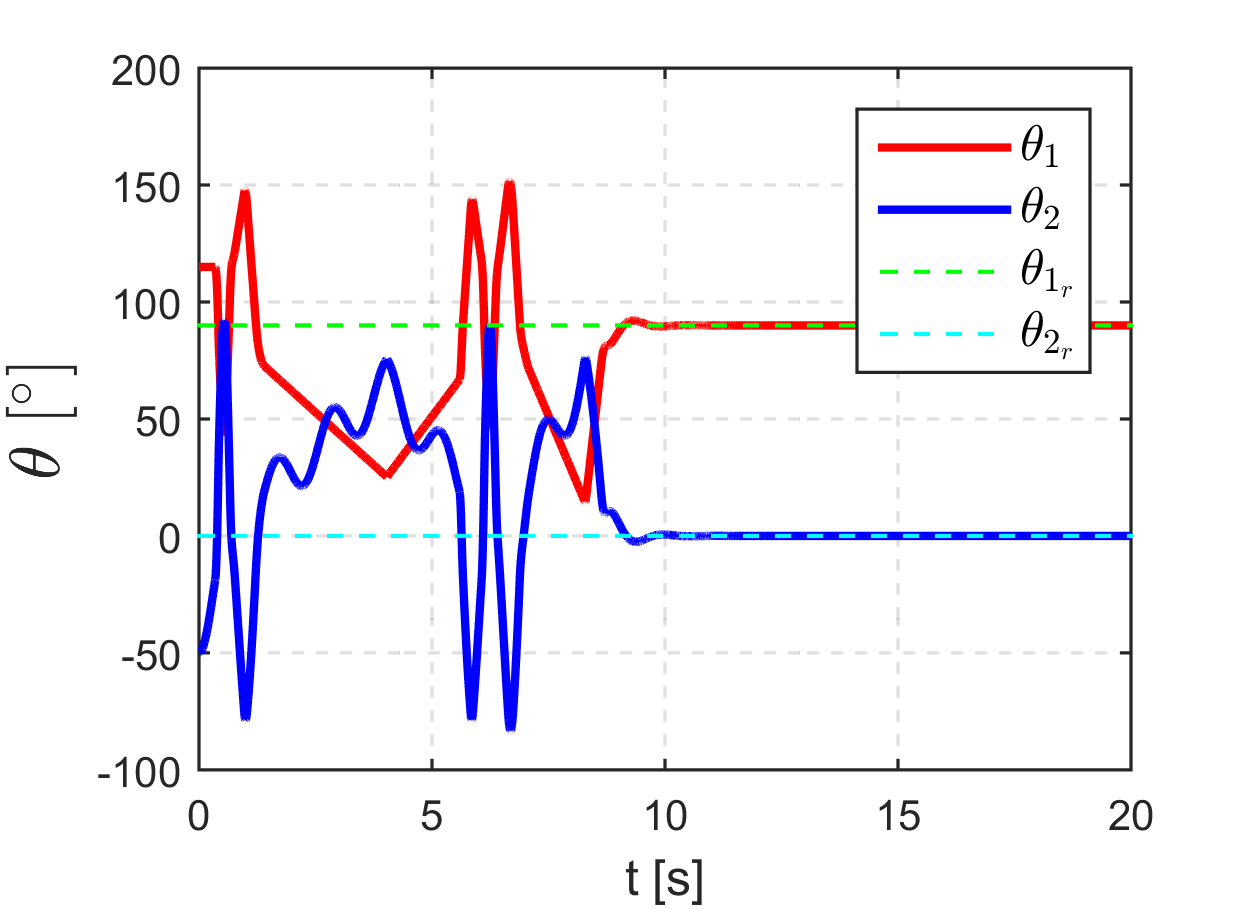
\includegraphics[width=0.85\linewidth]{img/pendubot_th1th2_z_sat}
	\caption{Angular positions of links -- Case II}
	\label{fig:re_pendu_th1th2_case_2}
\end{figure}
%
%
{\color{red} One can observe that the algorithm for Case~I ..............}


A wide range of  robotic application require an energy savings or restrictions on its expenditure  (through e.g. motors' finite power). 
As a consequence, the total energetic cost of driving the robot to the upright position was calculated during the simulation.
%
The dynamic effort criterion (\ref{eq:kryterium_energetyczne}) was used as an indicator of energy used by the algorithm. The effort was defined as
%
\begin{equation}
\label{eq:kryterium_energetyczne}
T = 
\int_0^{t_{max}} \tau^2 dt
\end{equation}
%
which is the integration of squares of all join torques over time \cite{human_motion_ksiazka}.
%
Figure~\ref{fig:re_pendu_tau}
% and Fig.~\ref{fig:re_pendu_tau_z_sat}
depicts the motor's torque expended during stabilization process for exemplary initial conditions.
%
%
\begin{figure}[!ht]
	\centering
	{\footnotesize a)}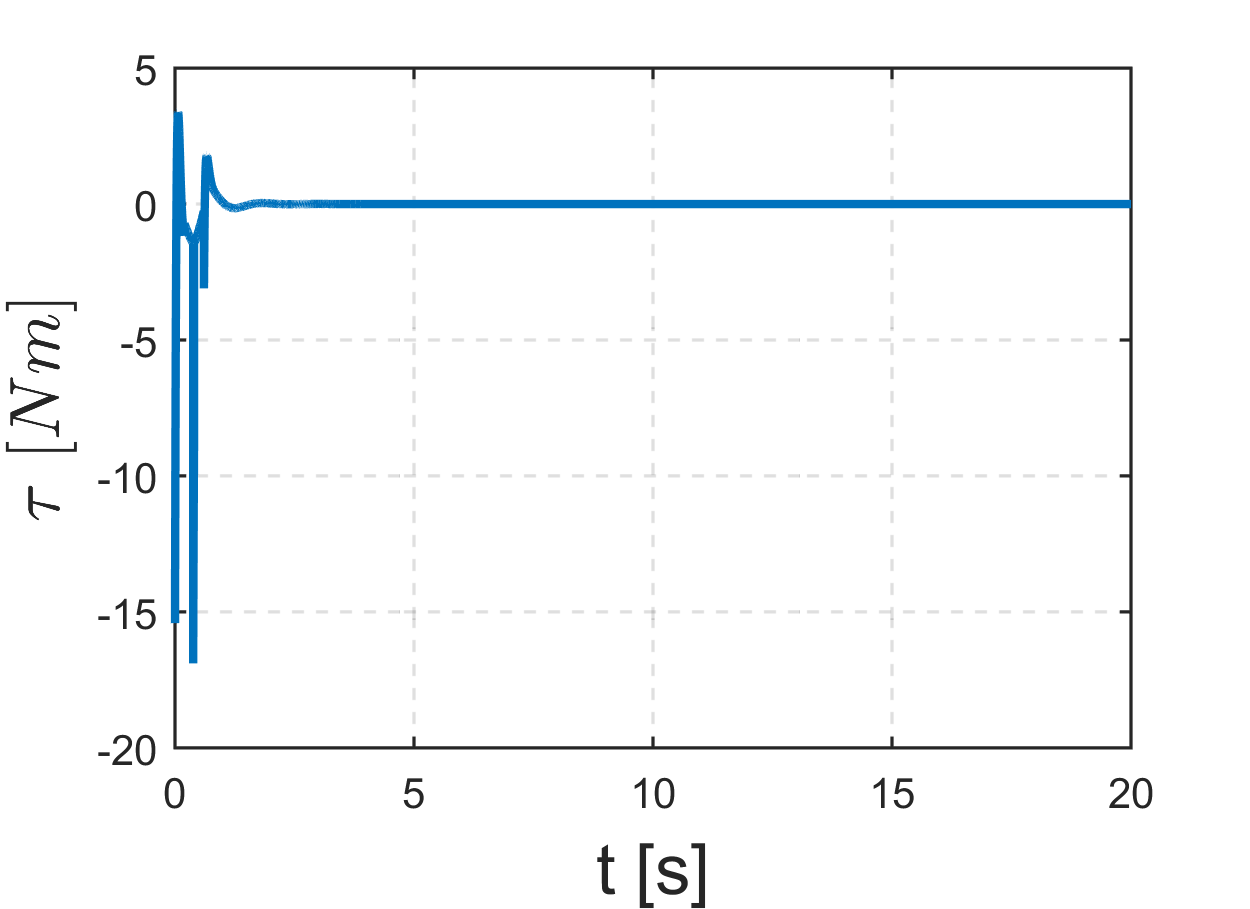
\includegraphics[width=0.46\linewidth]{img/tau_bez_sat}
	{\footnotesize b)}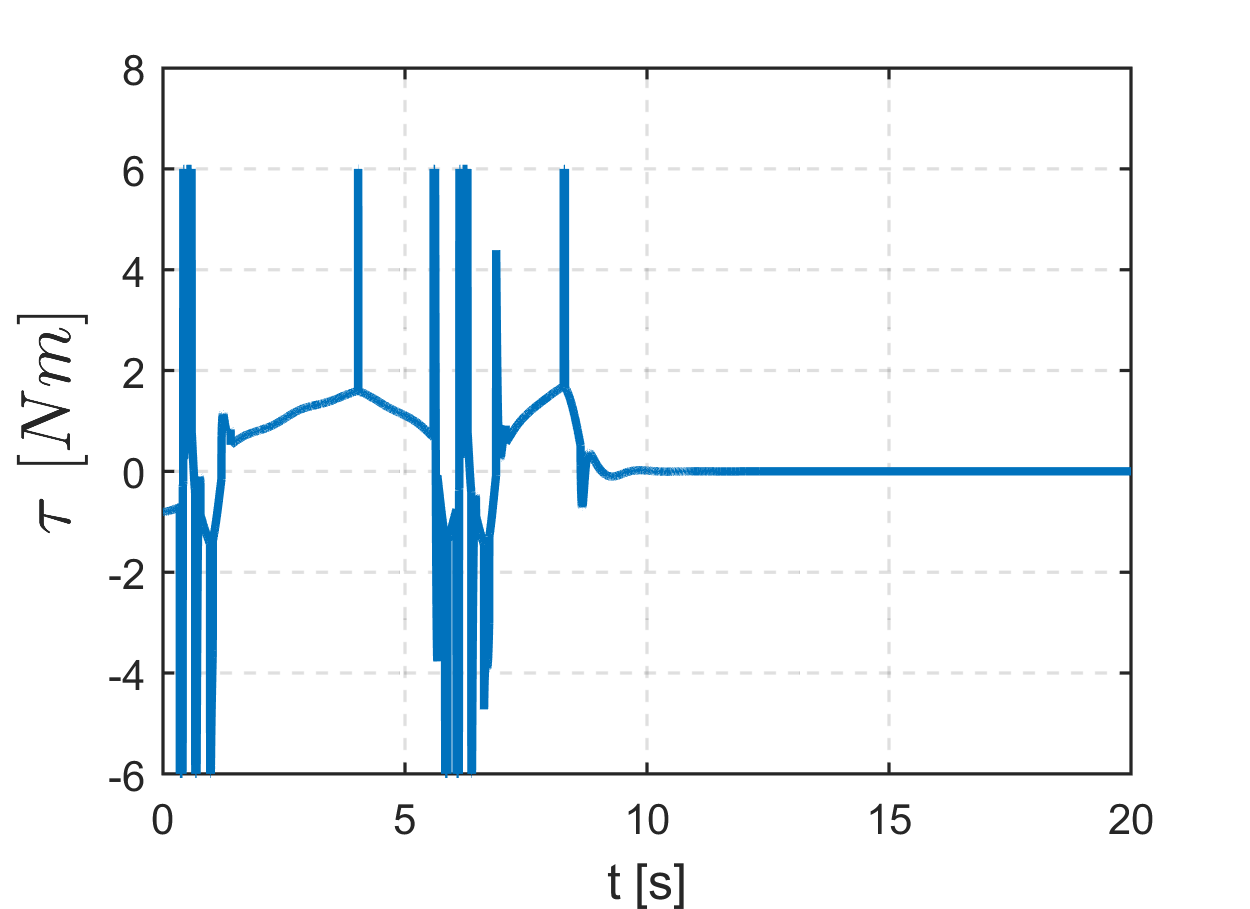
\includegraphics[width=0.46\linewidth]{img/tau_z_sat}
	\caption{Motor torque -- a) Case I, b) Case II}
	\label{fig:re_pendu_tau}
\end{figure}
%
%
%\begin{figure}[!ht]
%	\centering
%	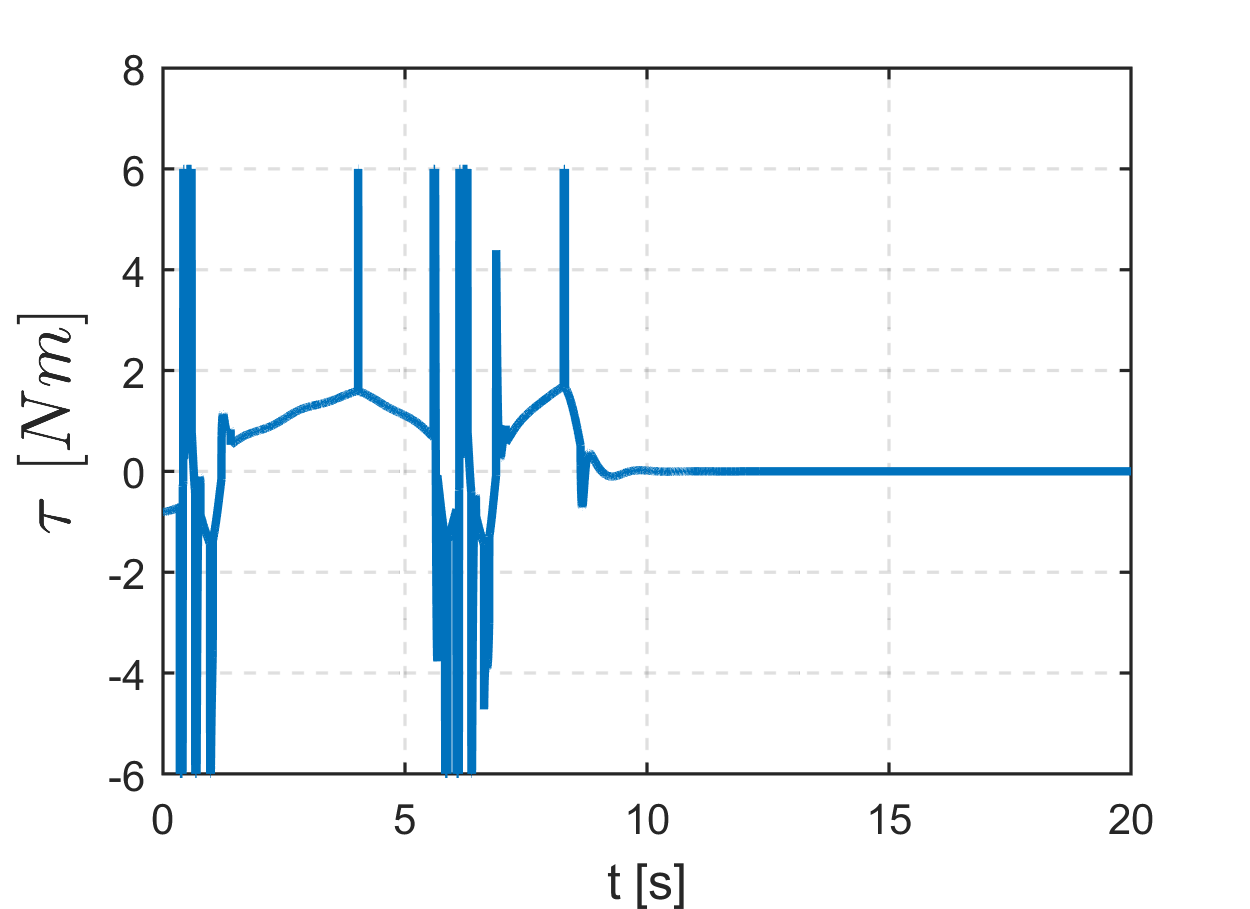
\includegraphics[width=0.9\linewidth]{img/tau_z_sat}
%	\caption{Motor torque -- Case II}
%	\label{fig:re_pendu_tau_z_sat}
%\end{figure}
%


The drawings depicting the total torque consumption during simulation are presented in Fig.~\ref{fig:re_pendu_tau_total_bez_sat} and Fig.~\ref{fig:re_pendu_tau_total_sat} for the Case~I and  Case~II, respectively.
%
\begin{figure}[!ht]
	\centering
	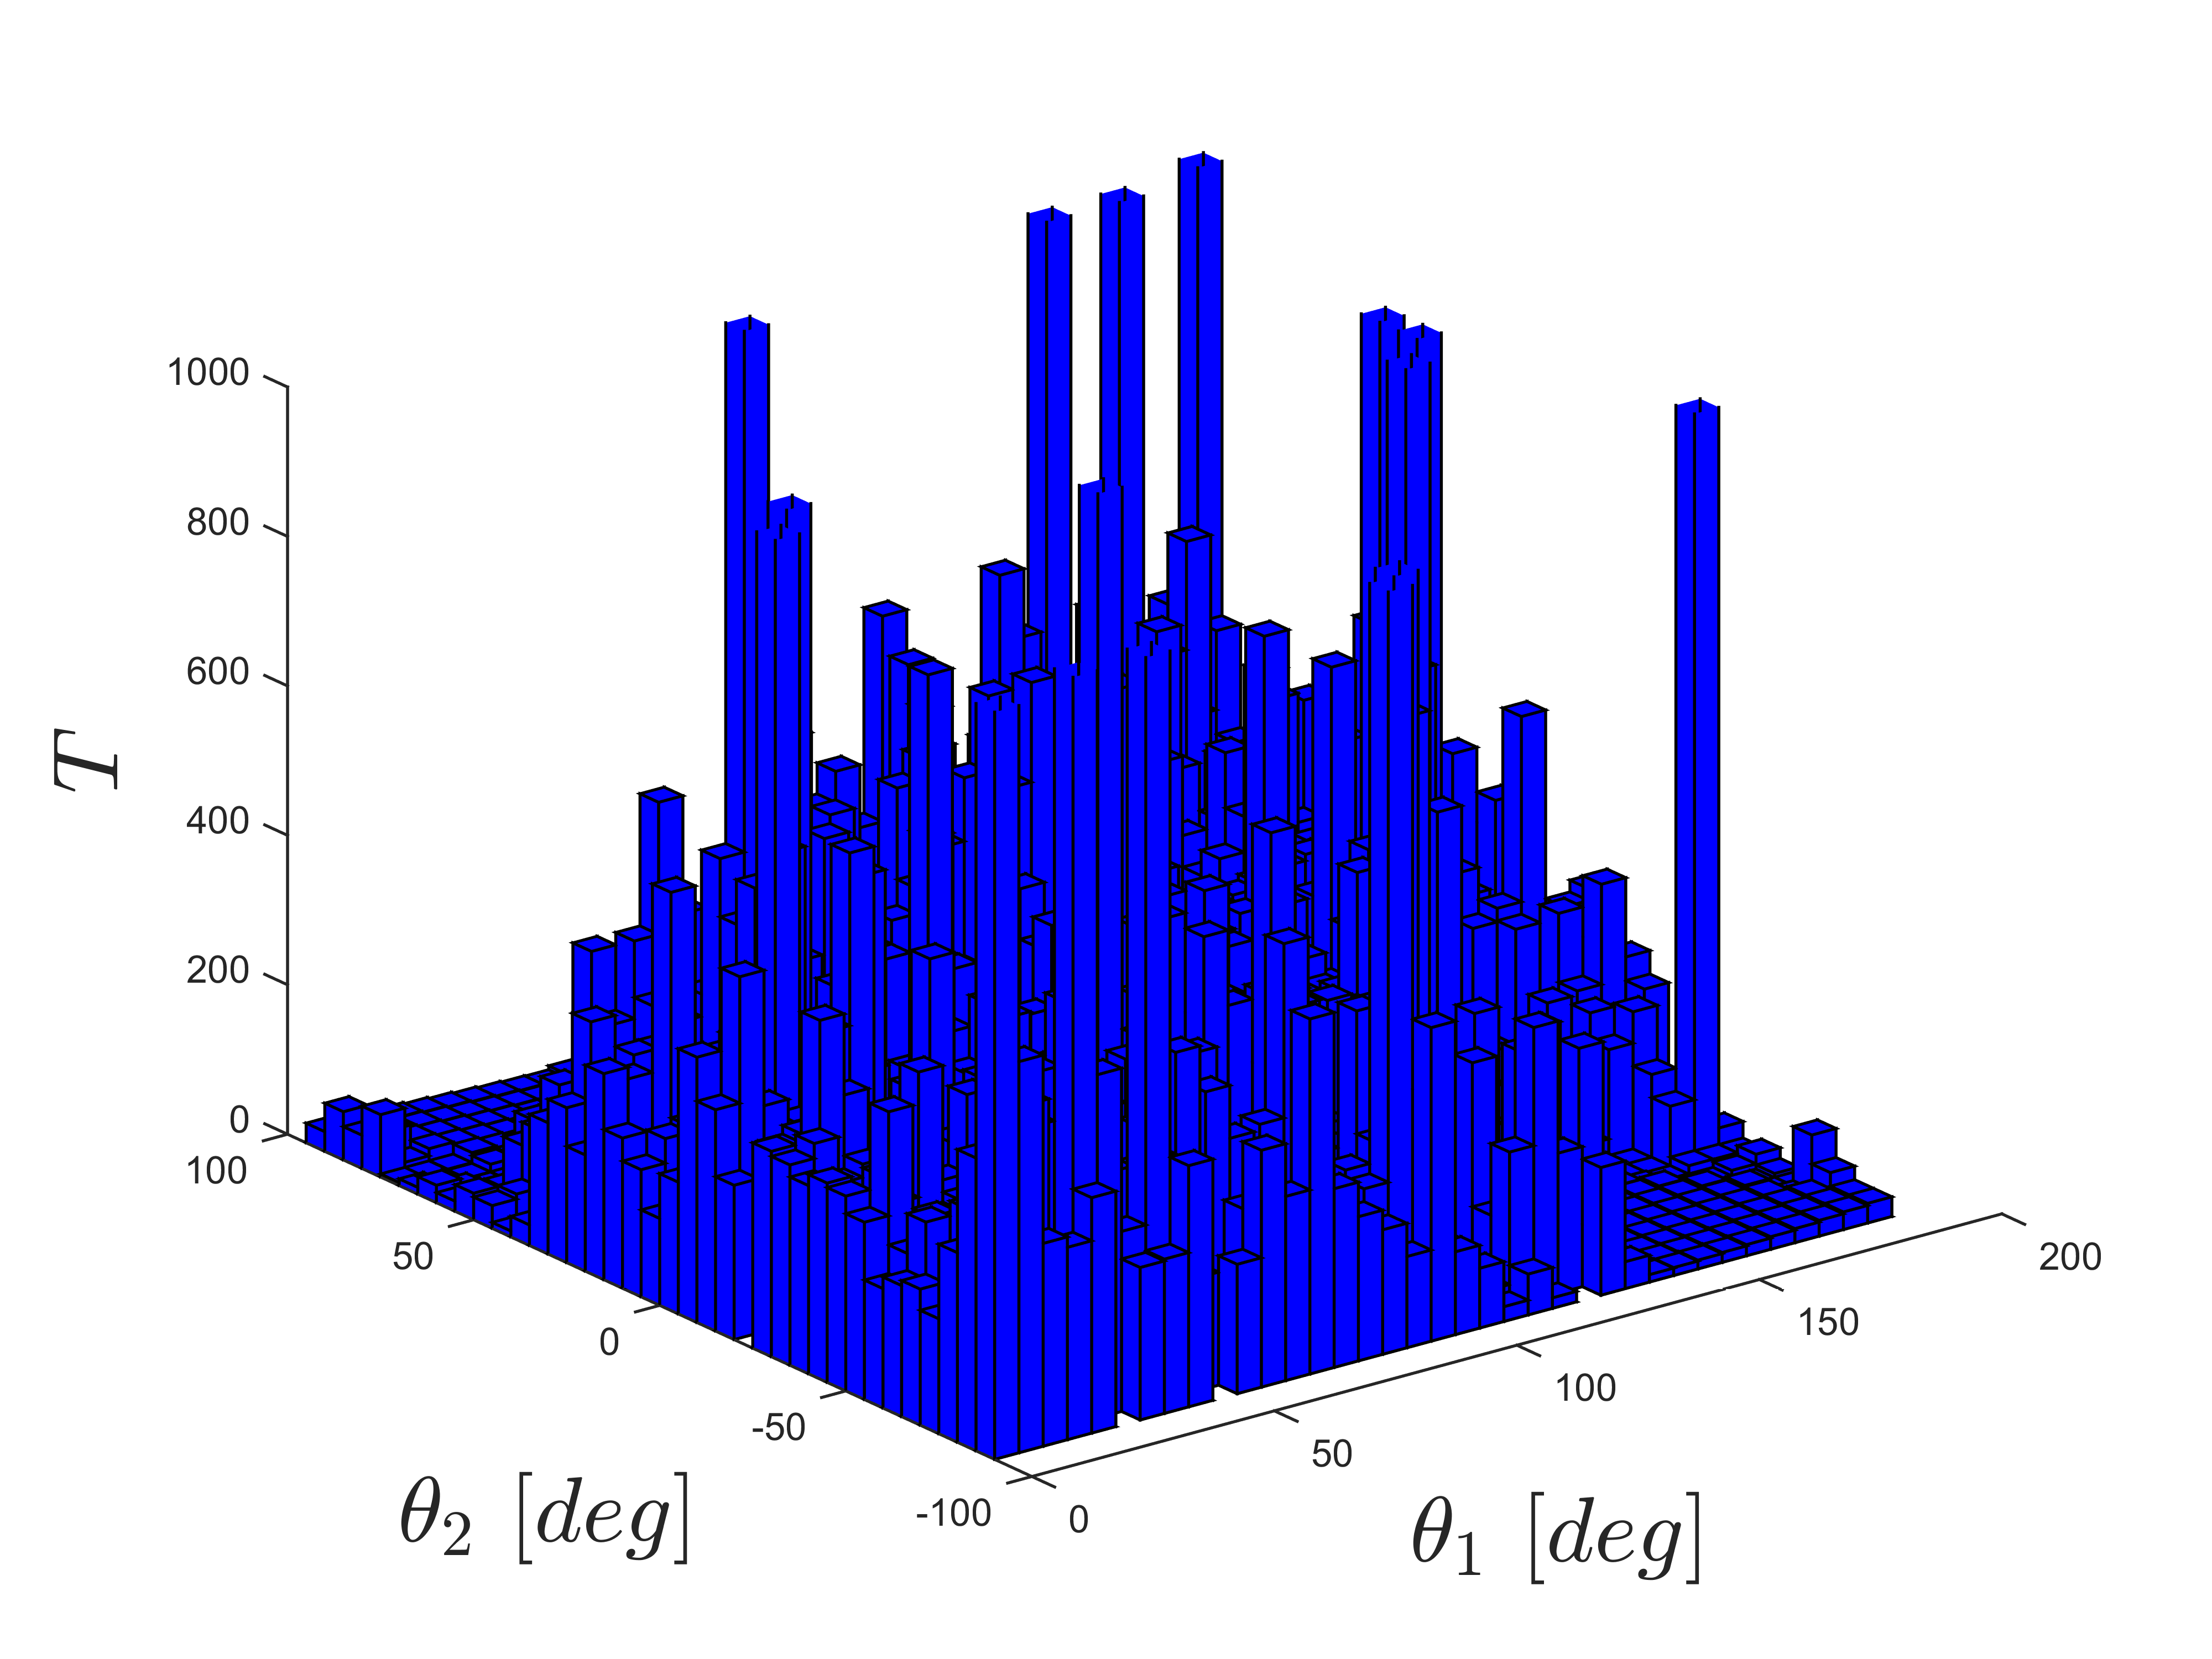
\includegraphics[width=0.93\linewidth]{img/RE_pendu_wykres_KE_bez_sat}
	\caption{Energetic cost of successful trials  -- Case I}
	\label{fig:re_pendu_tau_total_bez_sat}
\end{figure}
%
%
\begin{figure}[!ht]
	\centering
	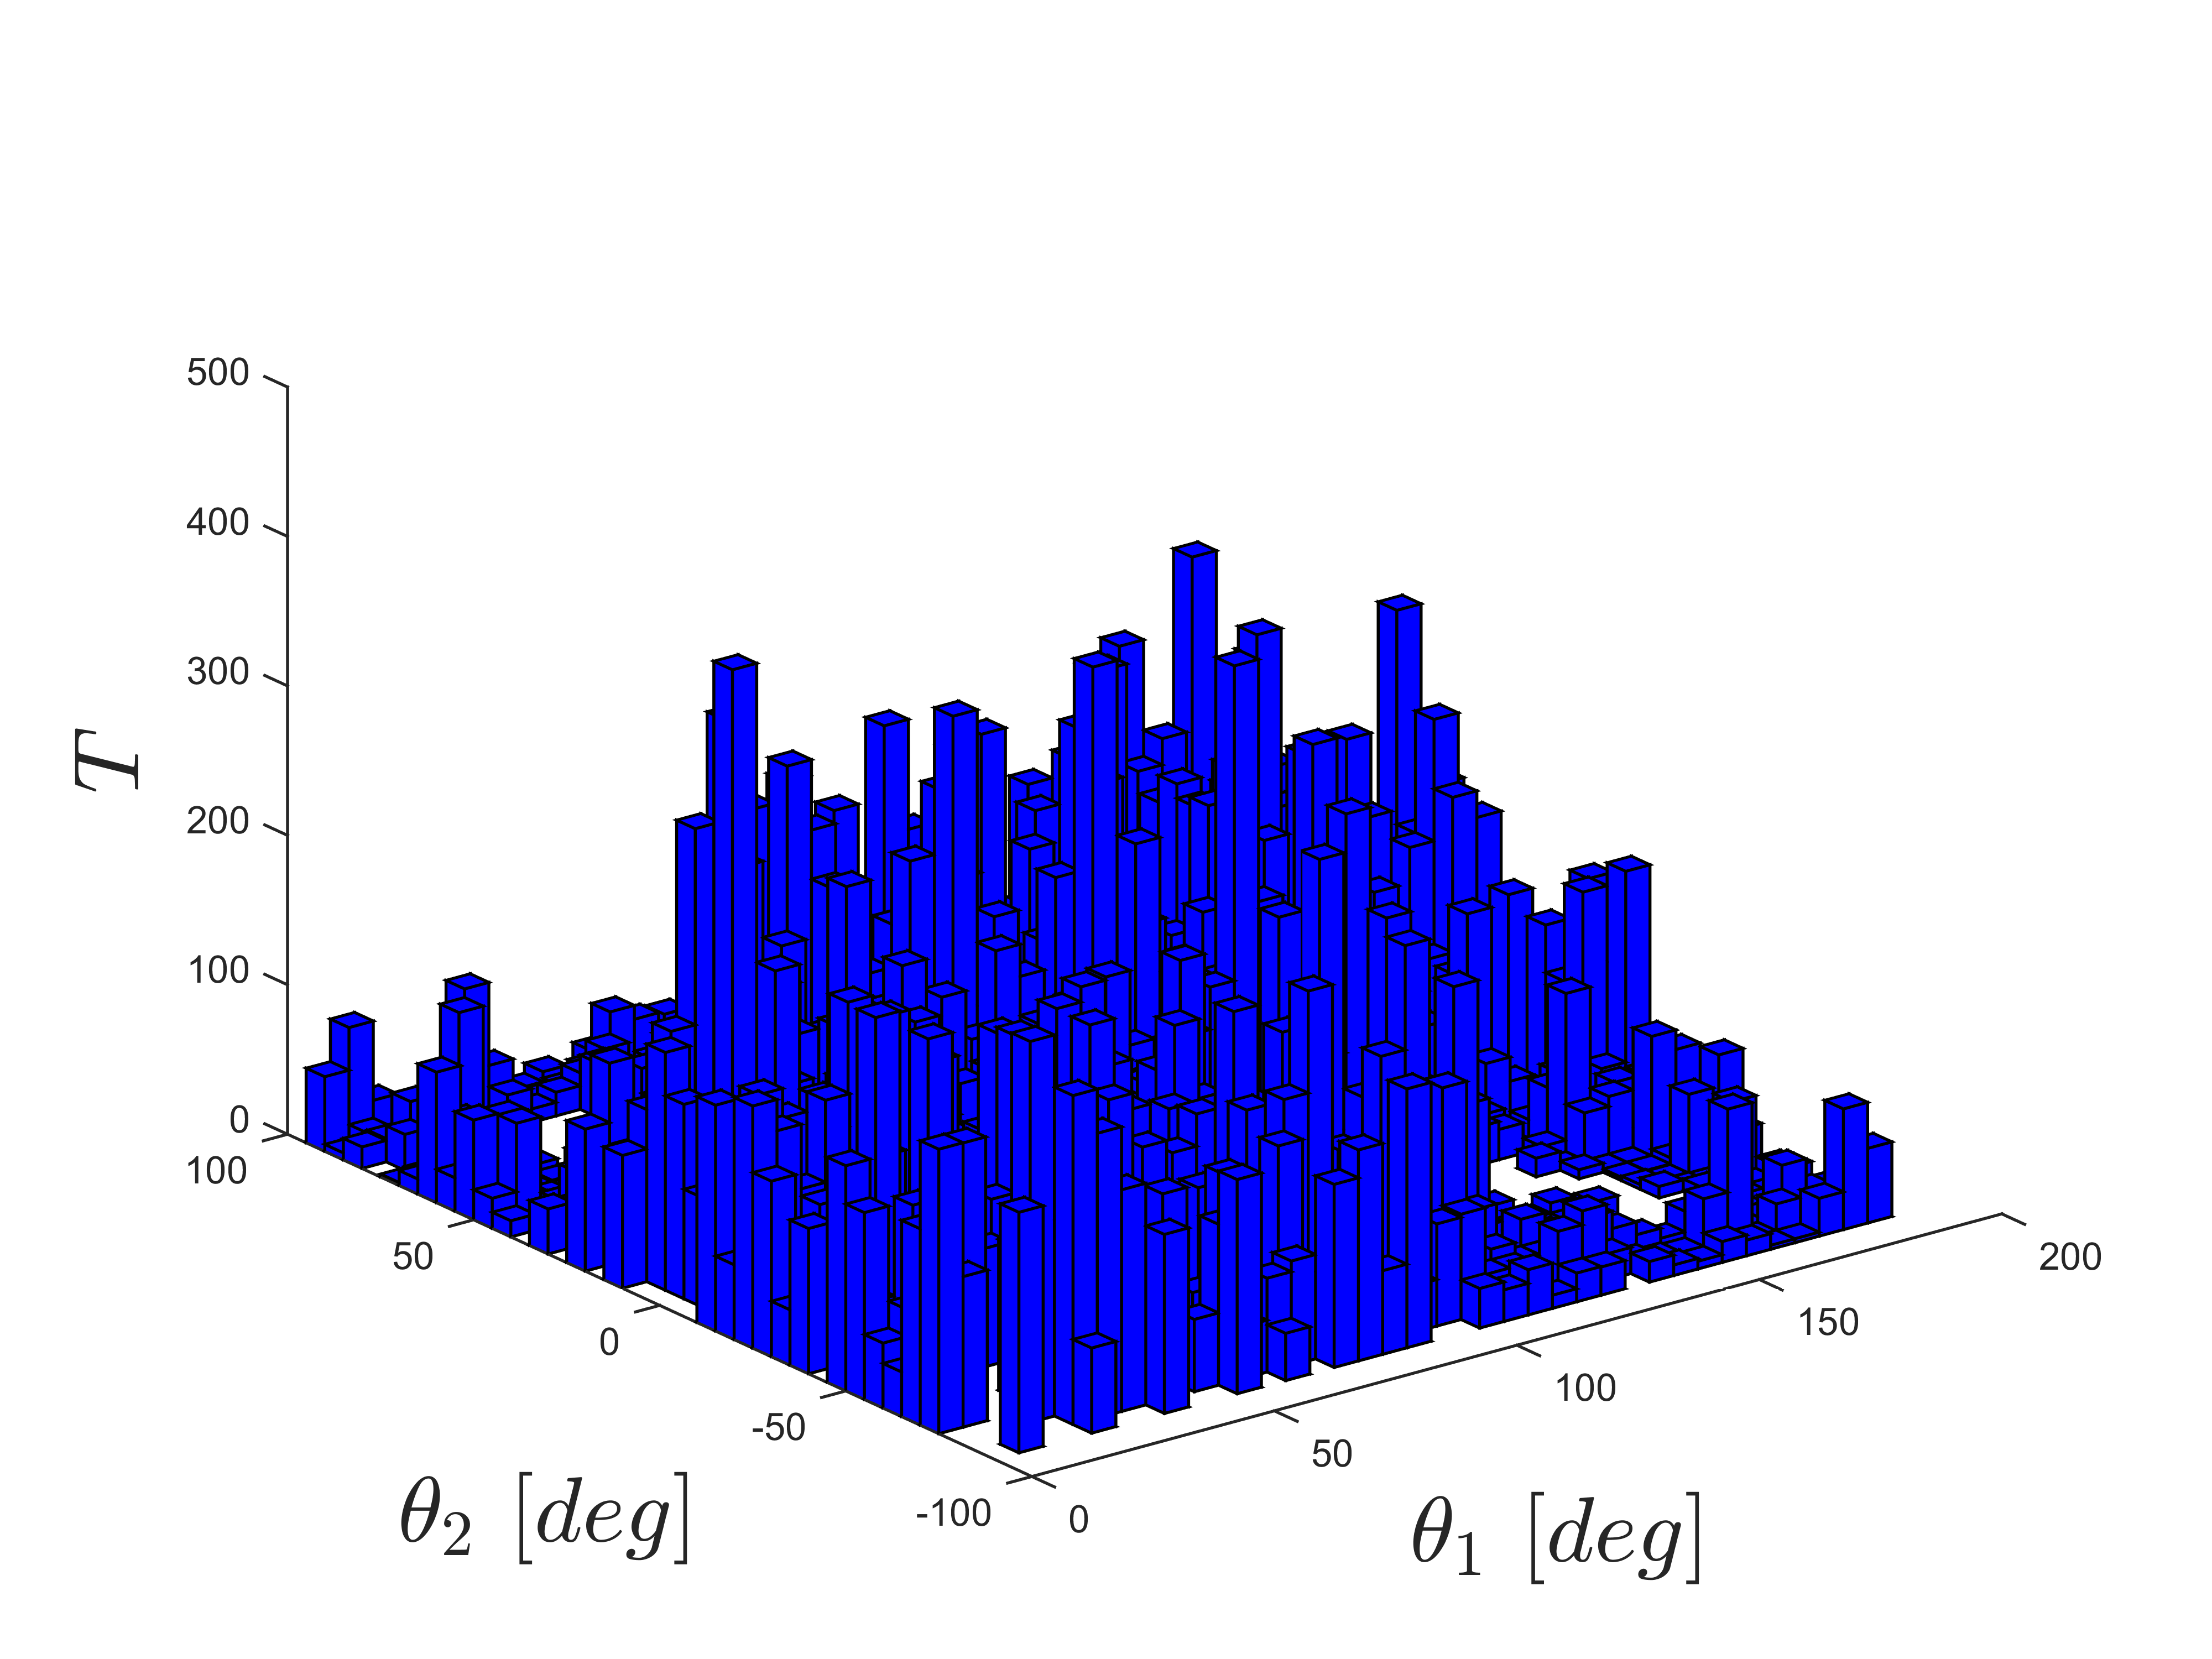
\includegraphics[width=0.93\linewidth]{img/RE_pendu_wykres_KE_sat}
	\caption{Energetic cost of successful trials  -- Case II}
	\label{fig:re_pendu_tau_total_sat}
\end{figure}
%
One can observe how the energy is being distributed over analyzed trials.
This observation can be useful to pick a specific trial with respect to energy consumption, to test the algorithm in a real robot, for example. 


Figure \ref{fig:re_pendu_reakcja_case} 
%and \ref{fig:re_pendu_reakcja_case_2} 
shows vertical component of ground reaction forces for exemplary successful trial.
One can observe that these values do not cross zero, which means that the robot does not lift-off during its movement.
%
%
\begin{figure}[!h]
\centering
{\footnotesize a)}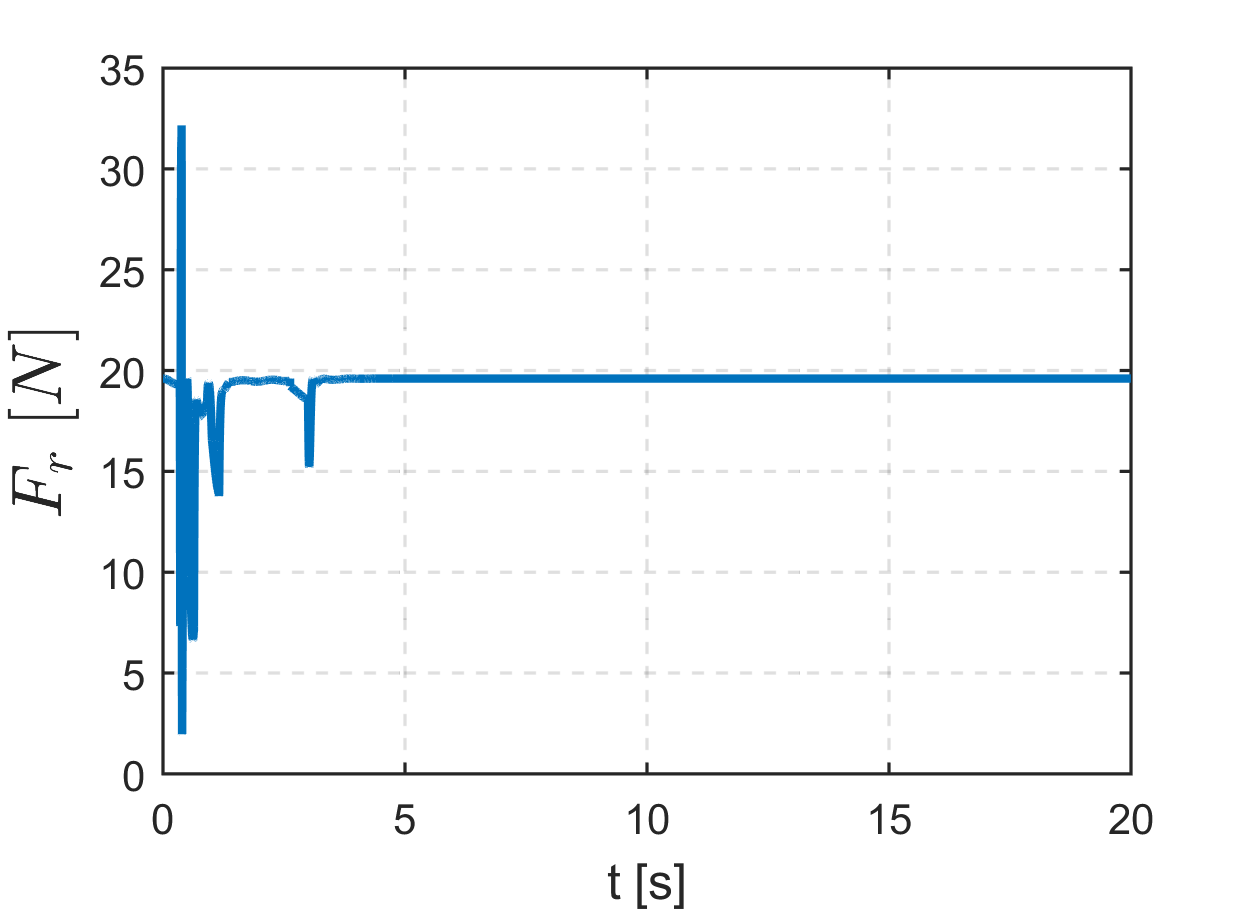
\includegraphics[width=0.46\linewidth]{img/Fr_bez_sat}
{\footnotesize b)}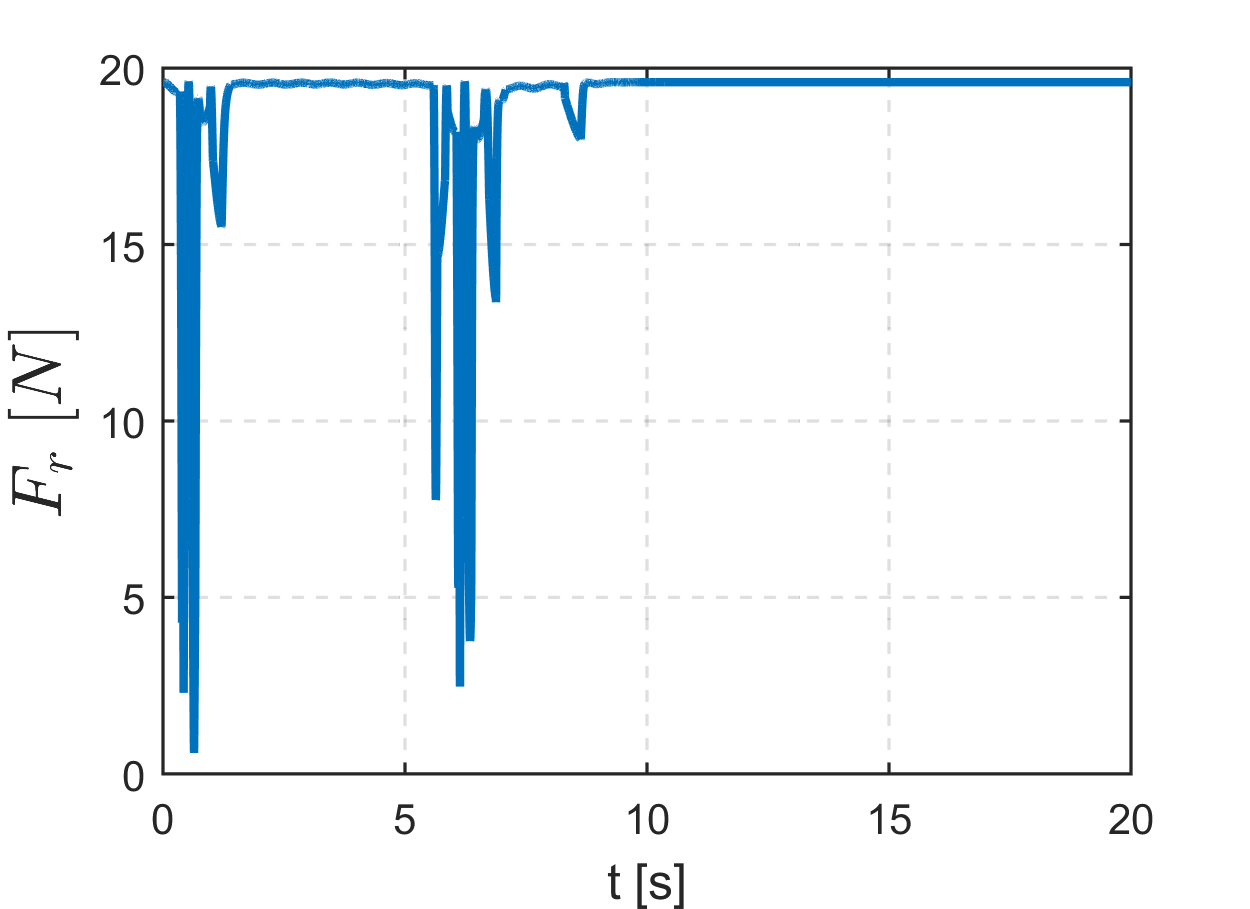
\includegraphics[width=0.46\linewidth]{img/Fr_z_sat}
\caption{Ground reaction forces -- a) Case I, b) Case II}
\label{fig:re_pendu_reakcja_case}
\end{figure}
%
%
%\begin{figure}[!h]
%	\centering
%	\caption{Ground reaction forces -- Case UI}
%	\label{fig:re_pendu_reakcja_case_2}
%\end{figure}
%%



%--------------------------------------------



% % % % % % % % % % % % % % % % % % % % % % % % % % % % % % % % % %


\section{Conclusion}
\label{sec:konkluzje}

The main objective of this paper was to present a simulation results of the new approach of controlling the Pendubot system.

One can draw a conclusion that analyzed approach is rather a representation of Pendubot's properties than an overall recipe  for stabilizing a double inverted pendulum with one actuation.
The algorithm does not guarantee that the system will not reach singularities.
One needs to impose several constraints in order to reflect the nature of the considered object as good as possible.
%
%
%\begin{ack}
%Place acknowledgments here.
%\end{ack}
%




\bibliographystyle{ifacconf-harvard}
\bibliography{bibliografia}


%\bibliographystyle{IEEEtran}
%\bibliography{mybibfile}







\end{document}
